% Some data/MC plots in control regions:
% - ttbar like region of ss2l
% - ttbar like region of 3l
% - ttZ/WZ like region of 3l

\subsection{Same-sign dilepton control plots}
Control regions are defined by selections similar to the signal region but with some reversed requirement to obtain background rich events. In case of same sign dilepton, the main background contribution from \ttbar\ is enhanced by requiring no untagged jet with $|\eta > 2|$. Furthermore, events with four or more jets are rejected to blind the signal region of the \ttH\ multilepton analysis. Some kinematic distributions in this control region for the same sign di-muon final state are shown in Fig.~\ref{fig:control_2lss_mumu}. Fig.~\ref{fig:control_2lss_emu} shows the distributions in case of \emu\ channel.
 \begin{figure} [!h]
  \centering
  \includegraphics[width=0.3\textwidth]{figures/controlplots/2lss-ttbar/mumu/Lep1Pt.pdf}
  \includegraphics[width=0.3\textwidth]{figures/controlplots/2lss-ttbar/mumu/Lep2Pt.pdf} 
  \includegraphics[width=0.3\textwidth]{figures/controlplots/2lss-ttbar/mumu/nJet25.pdf} \\
  \includegraphics[width=0.3\textwidth]{figures/controlplots/2lss-ttbar/mumu/nBJetLoose25.pdf} 
  \includegraphics[width=0.3\textwidth]{figures/controlplots/2lss-ttbar/mumu/minDRll.pdf}
  \includegraphics[width=0.3\textwidth]{figures/controlplots/2lss-ttbar/mumu/dPhiHighestPtSSPair.pdf} 
\caption{Contributions from signal and background in \ttbar\ control region for \mumu\ channel.}
\label{fig:control_2lss_mumu}
\end{figure}

 \begin{figure} [!h]
  \centering
  \includegraphics[width=0.3\textwidth]{figures/controlplots/2lss-ttbar/emu/Lep1Pt.pdf}
  \includegraphics[width=0.3\textwidth]{figures/controlplots/2lss-ttbar/emu/Lep2Pt.pdf}
  \includegraphics[width=0.3\textwidth]{figures/controlplots/2lss-ttbar/emu/nJet25.pdf} \\
  \includegraphics[width=0.3\textwidth]{figures/controlplots/2lss-ttbar/emu/nBJetLoose25.pdf}
  \includegraphics[width=0.3\textwidth]{figures/controlplots/2lss-ttbar/emu/minDRll.pdf}
  \includegraphics[width=0.3\textwidth]{figures/controlplots/2lss-ttbar/emu/dPhiHighestPtSSPair.pdf}
\caption{Contributions from signal and background in \ttbar\ control region for \emu\ channel.}
\label{fig:control_2lss_emu}
\end{figure}

\subsection{Three lepton control plots}
\paragraph{\Z-enriched sideband}
We first enrich the signal region in \WZ\ and \ttZ\ events by inverting the \Z\ veto of Tab.~\ref{tab:evsel}, \ie\ by requiring an opposite-sign dilepton pair with $|m_{\ell\ell}-m_\Z < 15\GeV|$.
To increase the available statistics, only a loose CSV jet is required (rather than a medium tagged one, as in Tab.~\ref{tab:evsel}).
A few relevant kinematic distributions shown in Fig.~\ref{fig:3lzcontrol} show a good overall agreement, albeit with a deficit of data at low momenta of the third lepton.
\begin{figure} [!h]
  \centering
  \includegraphics[width=0.30\textwidth]{figures/controlplots/3l-Z/Lep1Pt.pdf}
  \includegraphics[width=0.30\textwidth]{figures/controlplots/3l-Z/Lep2Pt.pdf}
  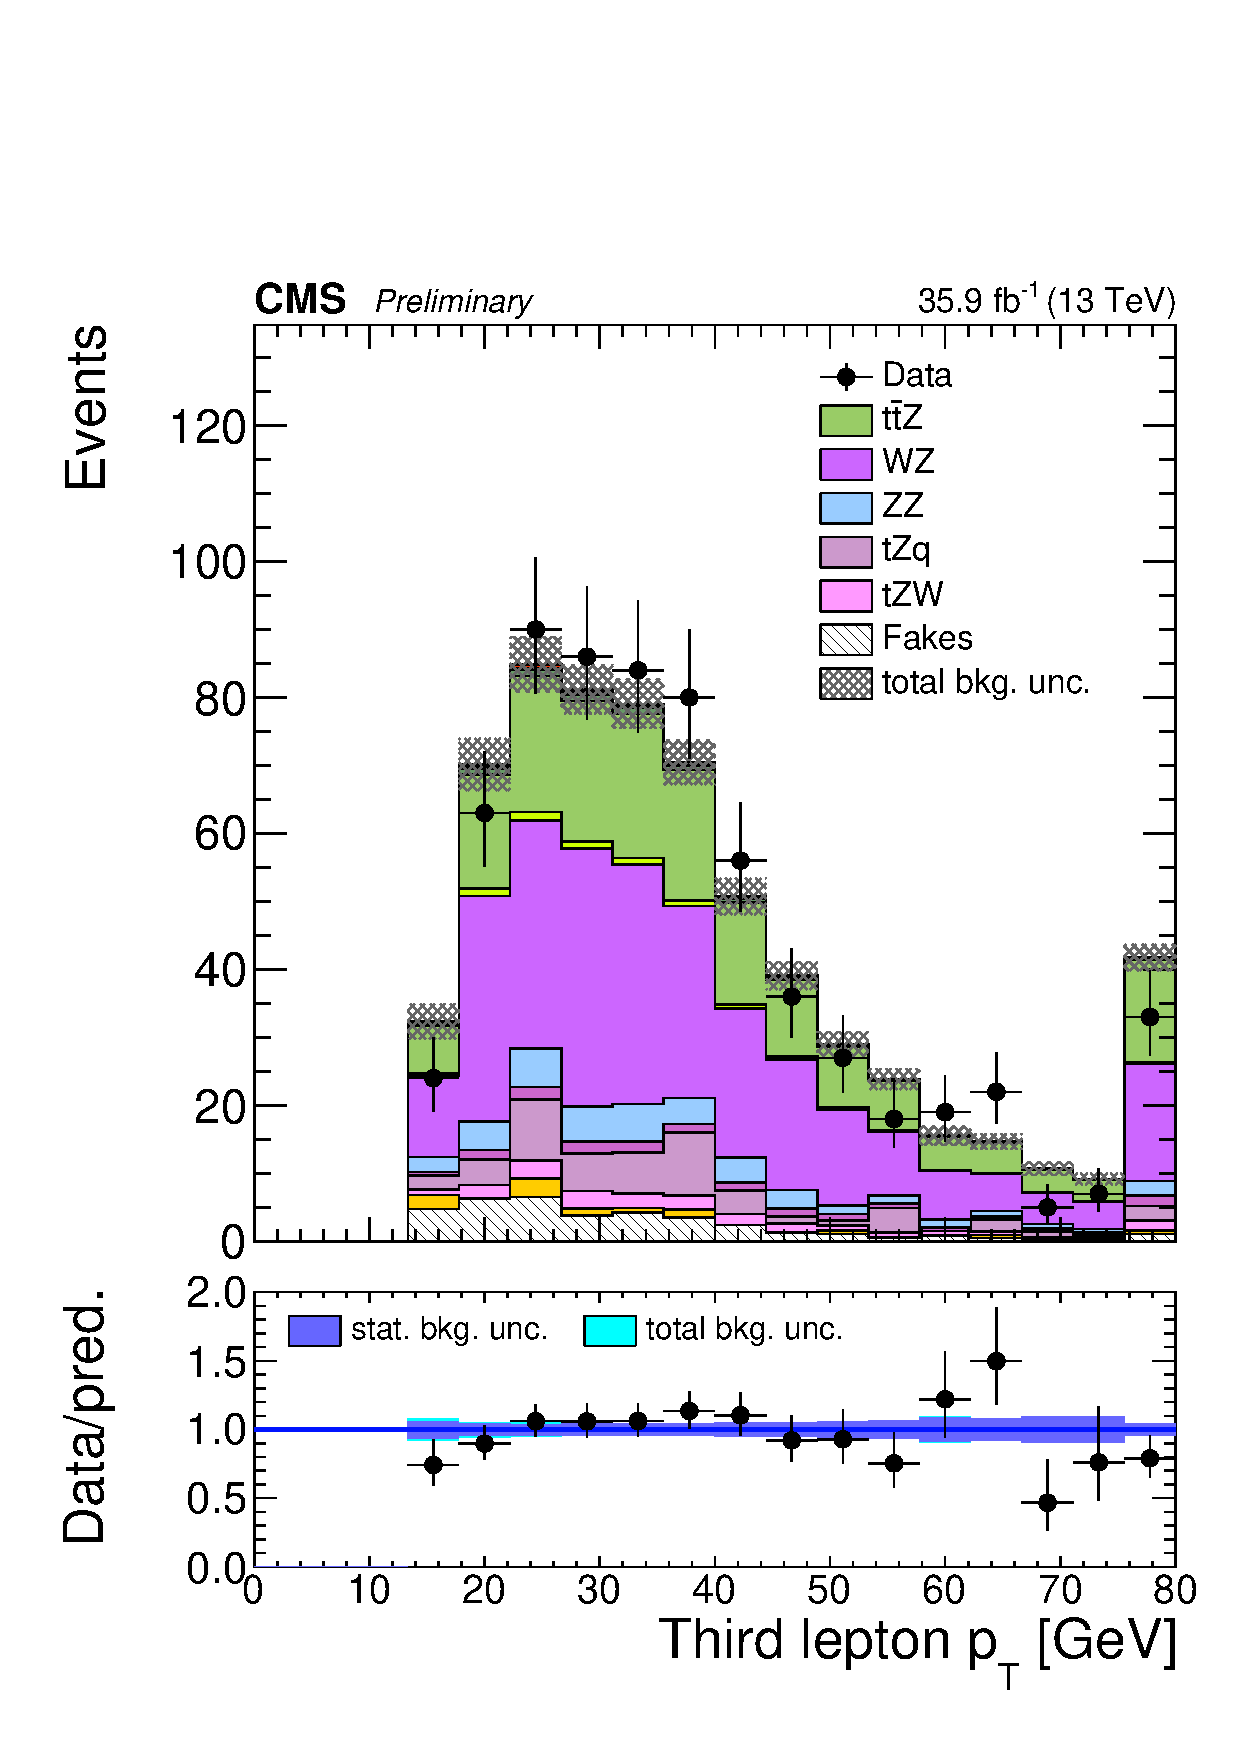
\includegraphics[width=0.30\textwidth]{figures/controlplots/3l-Z/Lep3Pt.pdf} \\
  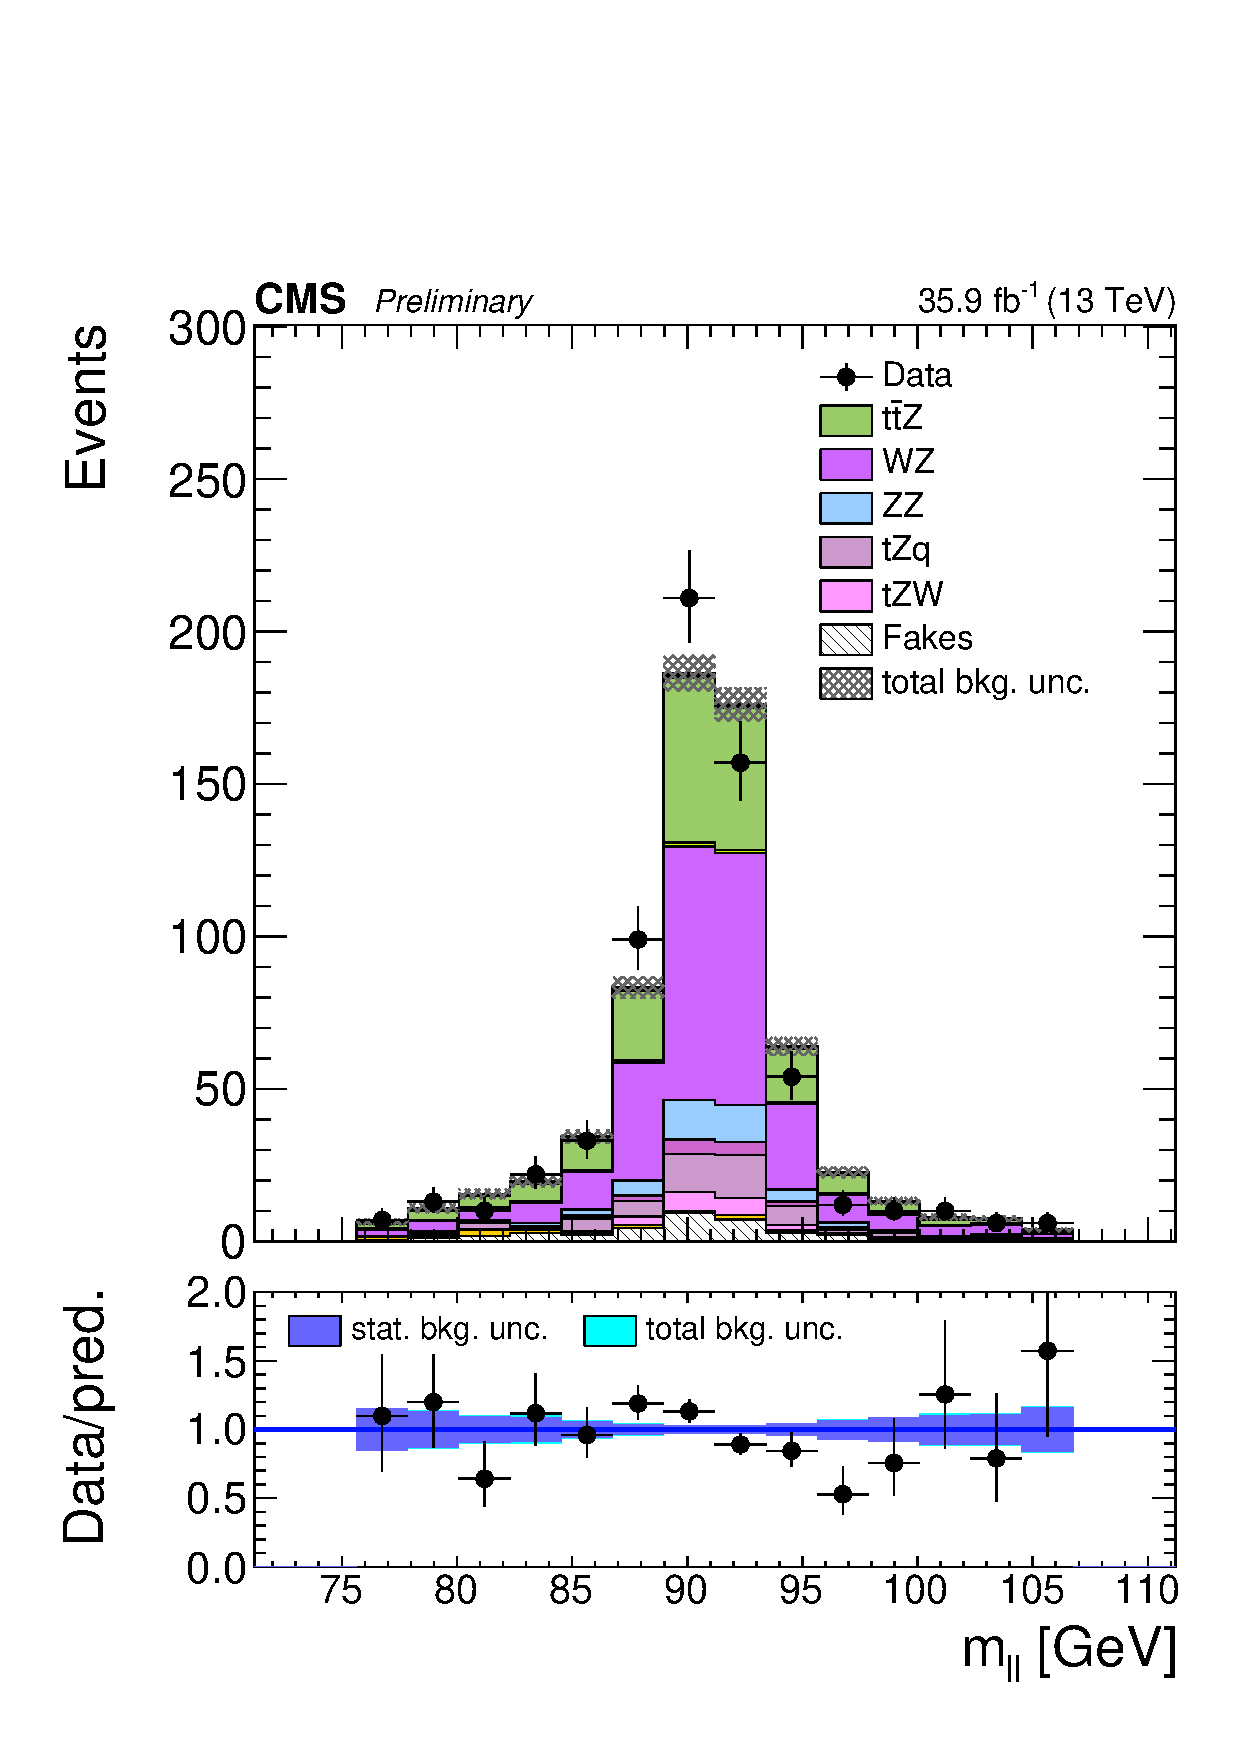
\includegraphics[width=0.30\textwidth]{figures/controlplots/3l-Z/mZ1.pdf}
  \includegraphics[width=0.30\textwidth]{figures/controlplots/3l-Z/nBJetLoose25.pdf}
  \includegraphics[width=0.30\textwidth]{figures/controlplots/3l-Z/nJet25.pdf} 
\caption{Kinematic distributions in the \Z-enriched sideband to the three-lepton signal region.}
\label{fig:3lzcontrol}
\end{figure}

%% Commented out since it has large overlap with the ttH signal region
% \paragraph{Background dominated}
% To study a selection closer to the signal region, we reject events with a light forward jet with $\eta>2$, and increase the available statistics with loosening the selection on the \cPqb-tagged jet to be CSV loose rather than CSV medium.
% Some relevant kinematic quantities of this event sample are shown in Fig.~\ref{fig:3lttcontrol}, showing excellent agreement with expectations.
% \begin{figure} [!h]
%   \centering
%   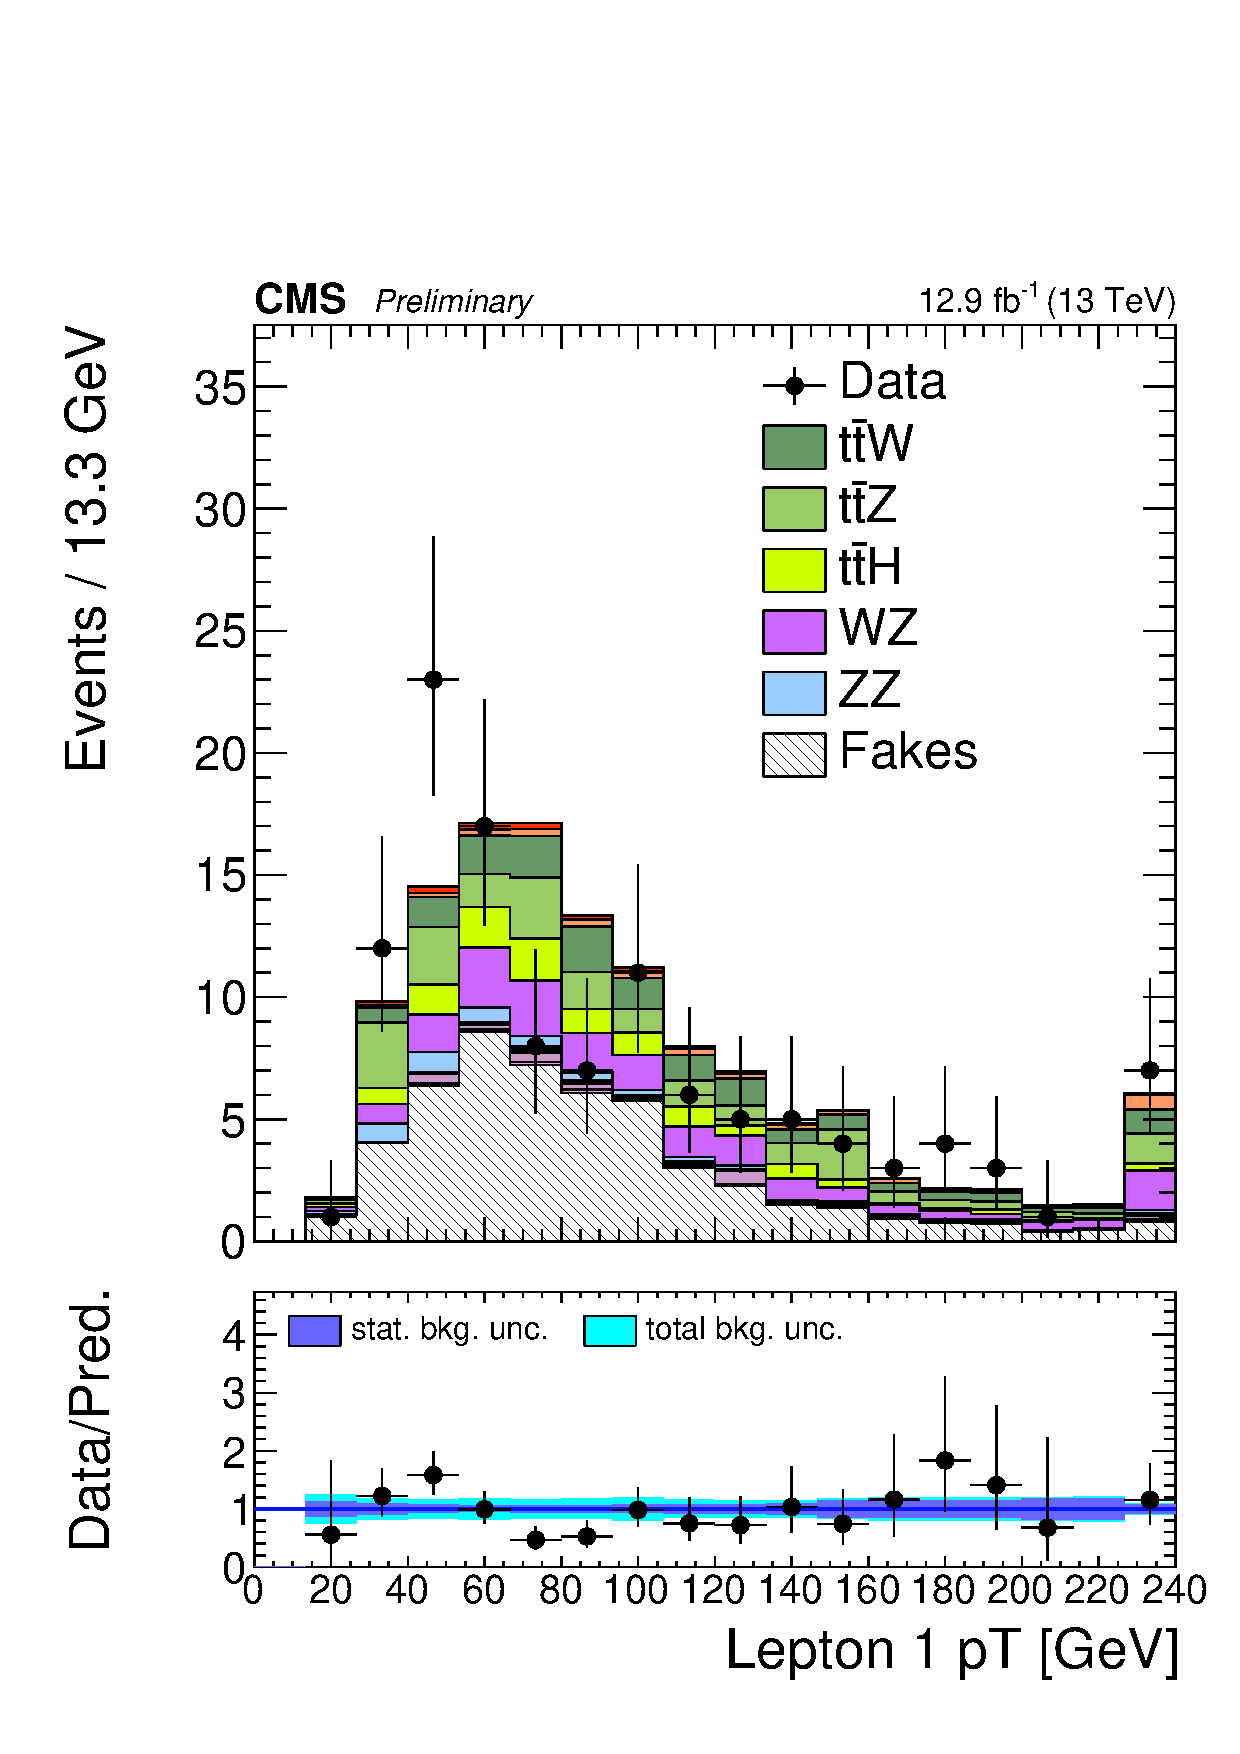
\includegraphics[width=0.30\textwidth]{figures/controlplots/3l-ttbar/Lep1ConePt.pdf}
%   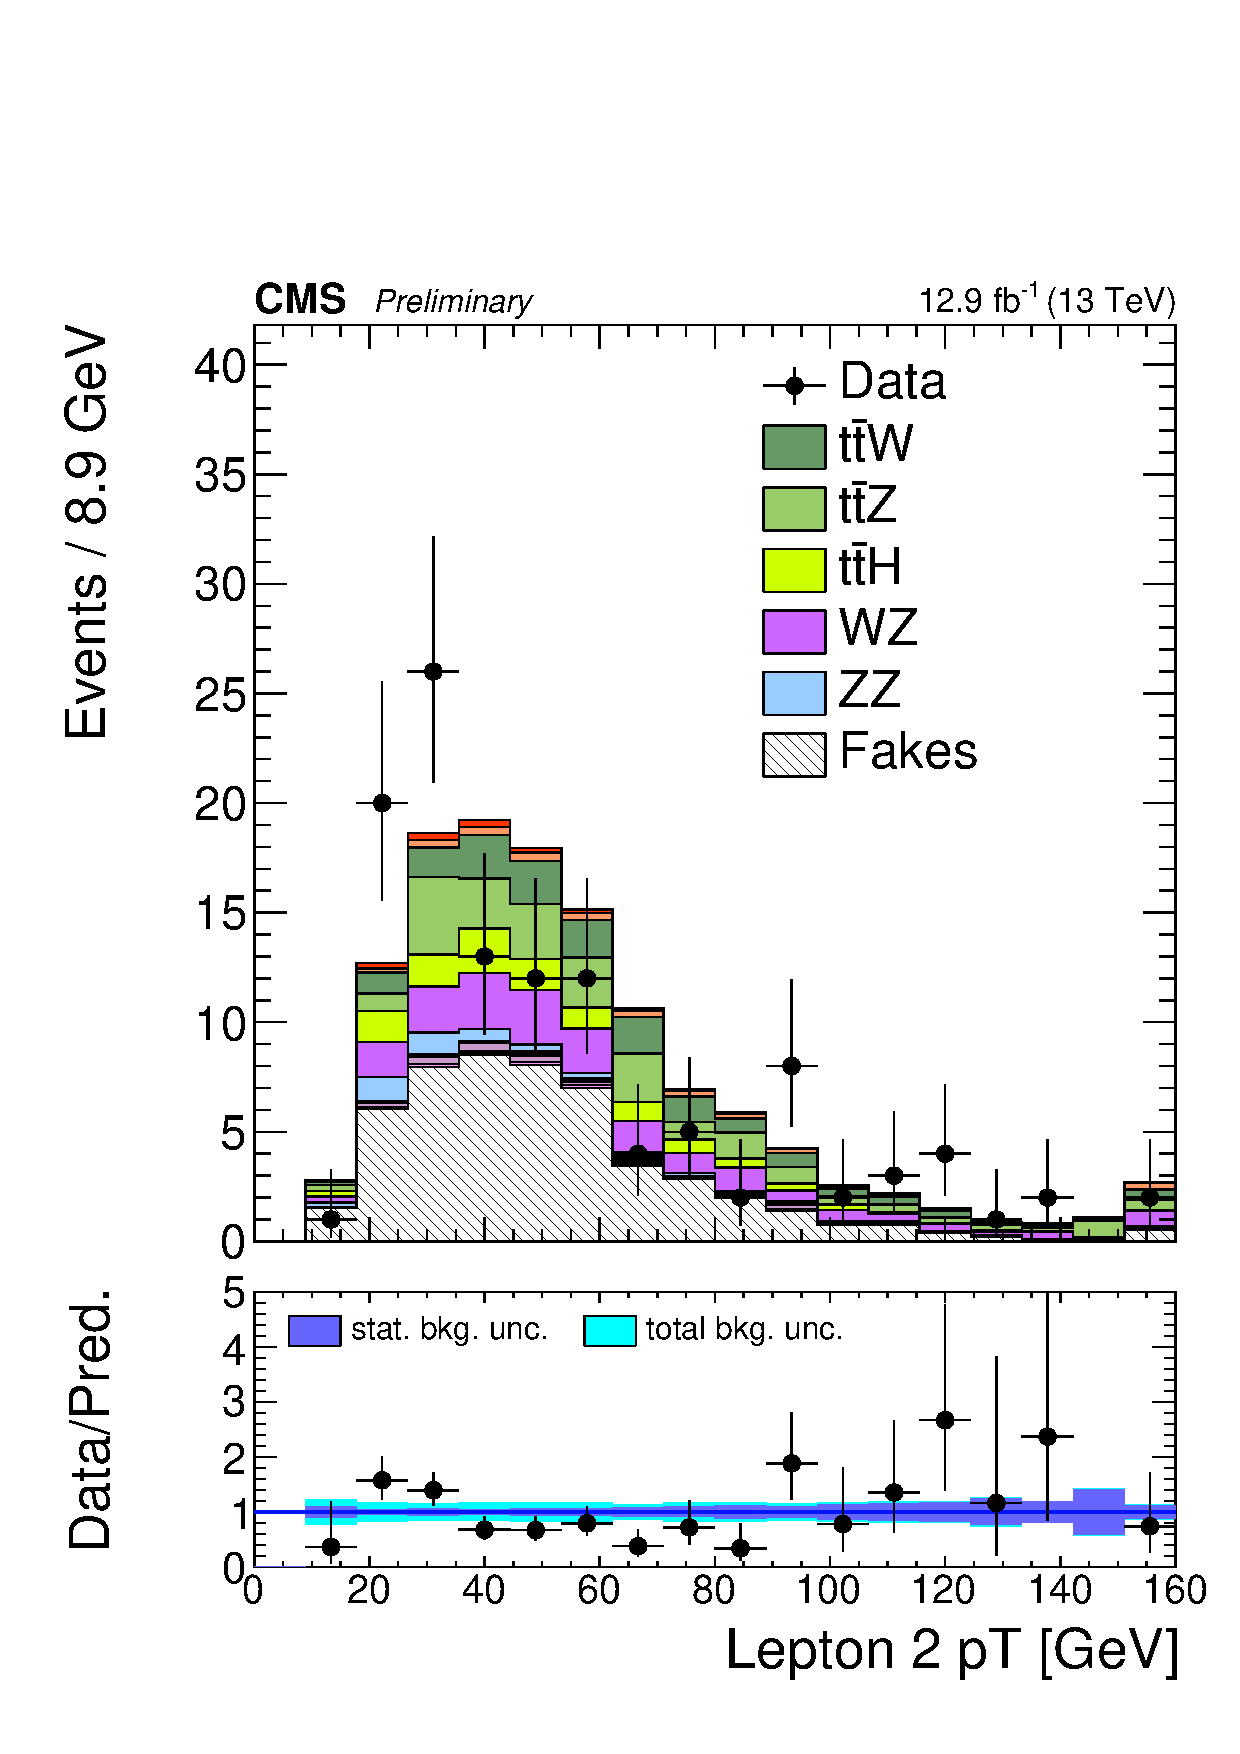
\includegraphics[width=0.30\textwidth]{figures/controlplots/3l-ttbar/Lep2ConePt.pdf}
%   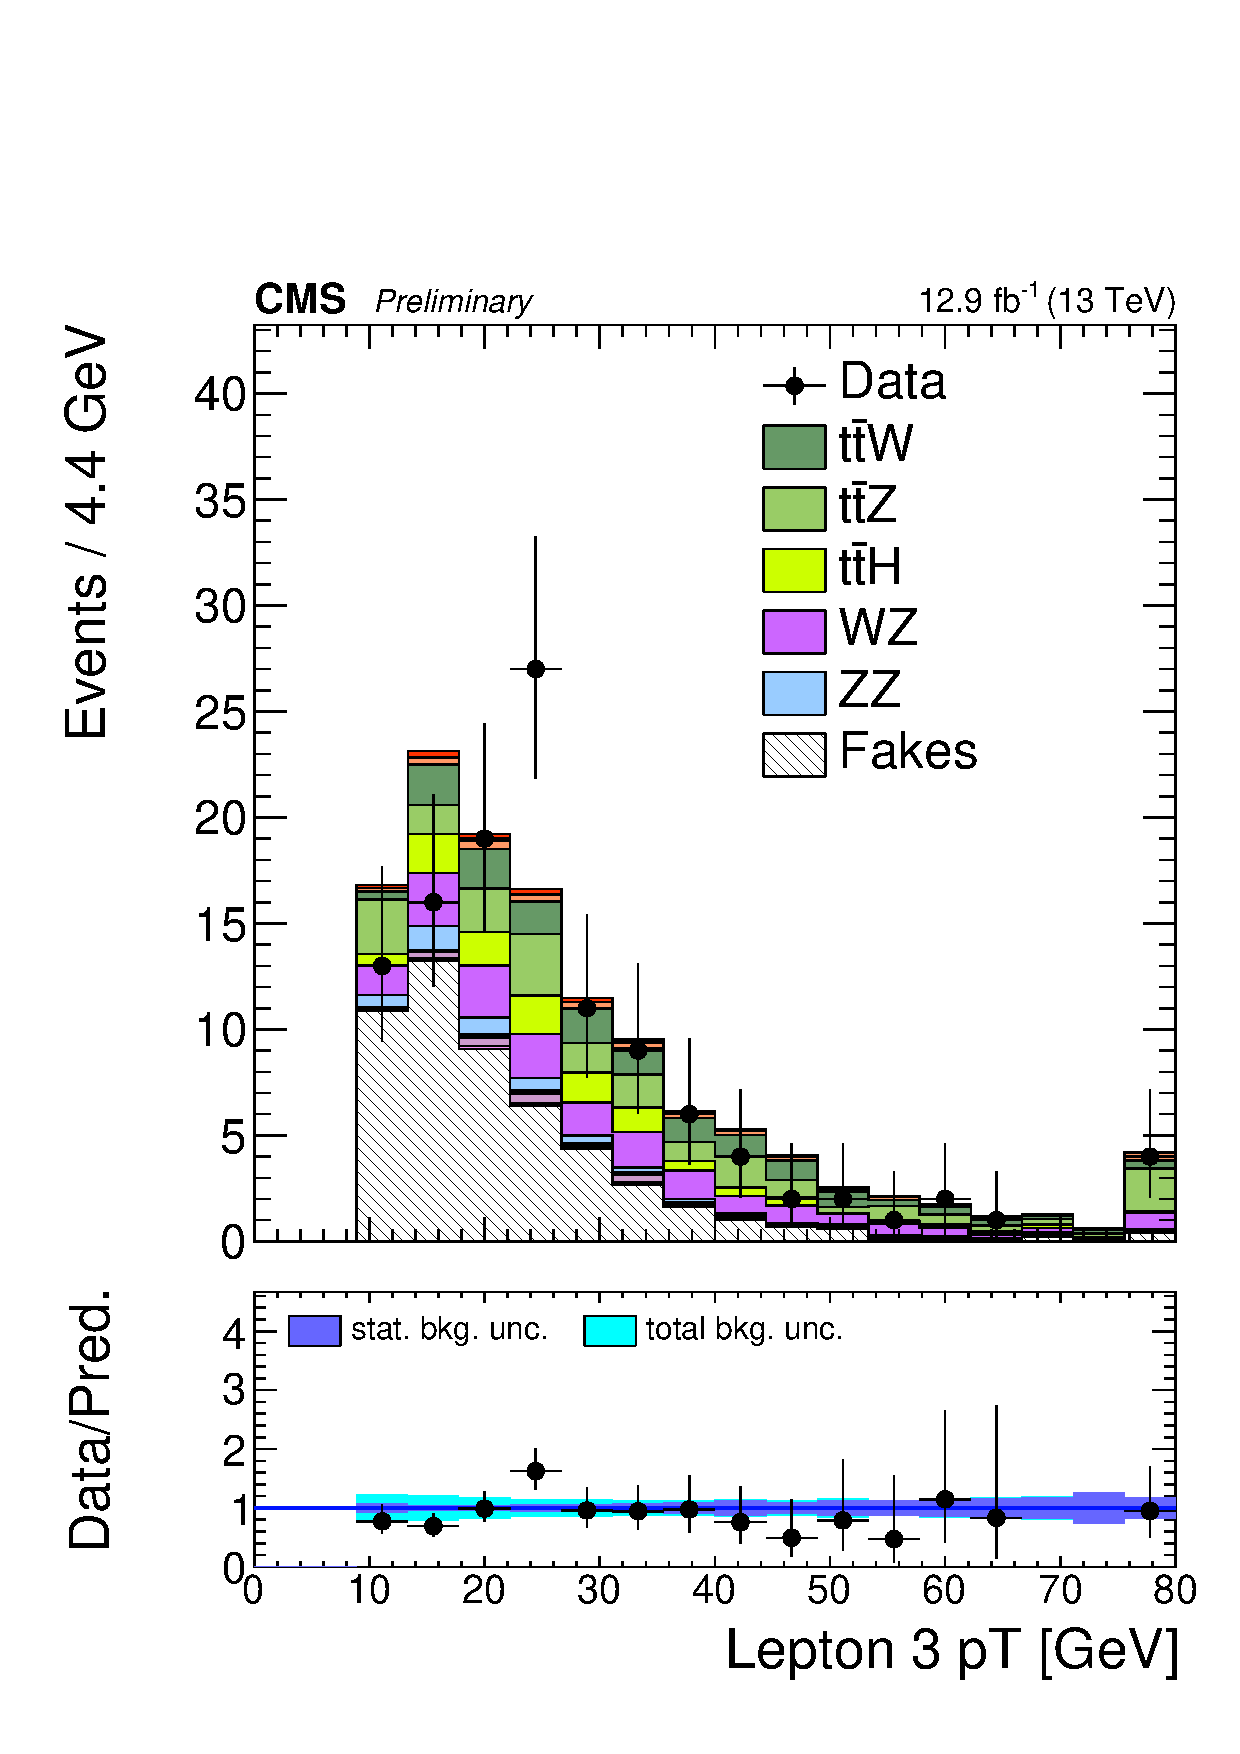
\includegraphics[width=0.30\textwidth]{figures/controlplots/3l-ttbar/Lep3ConePt.pdf} \\
%   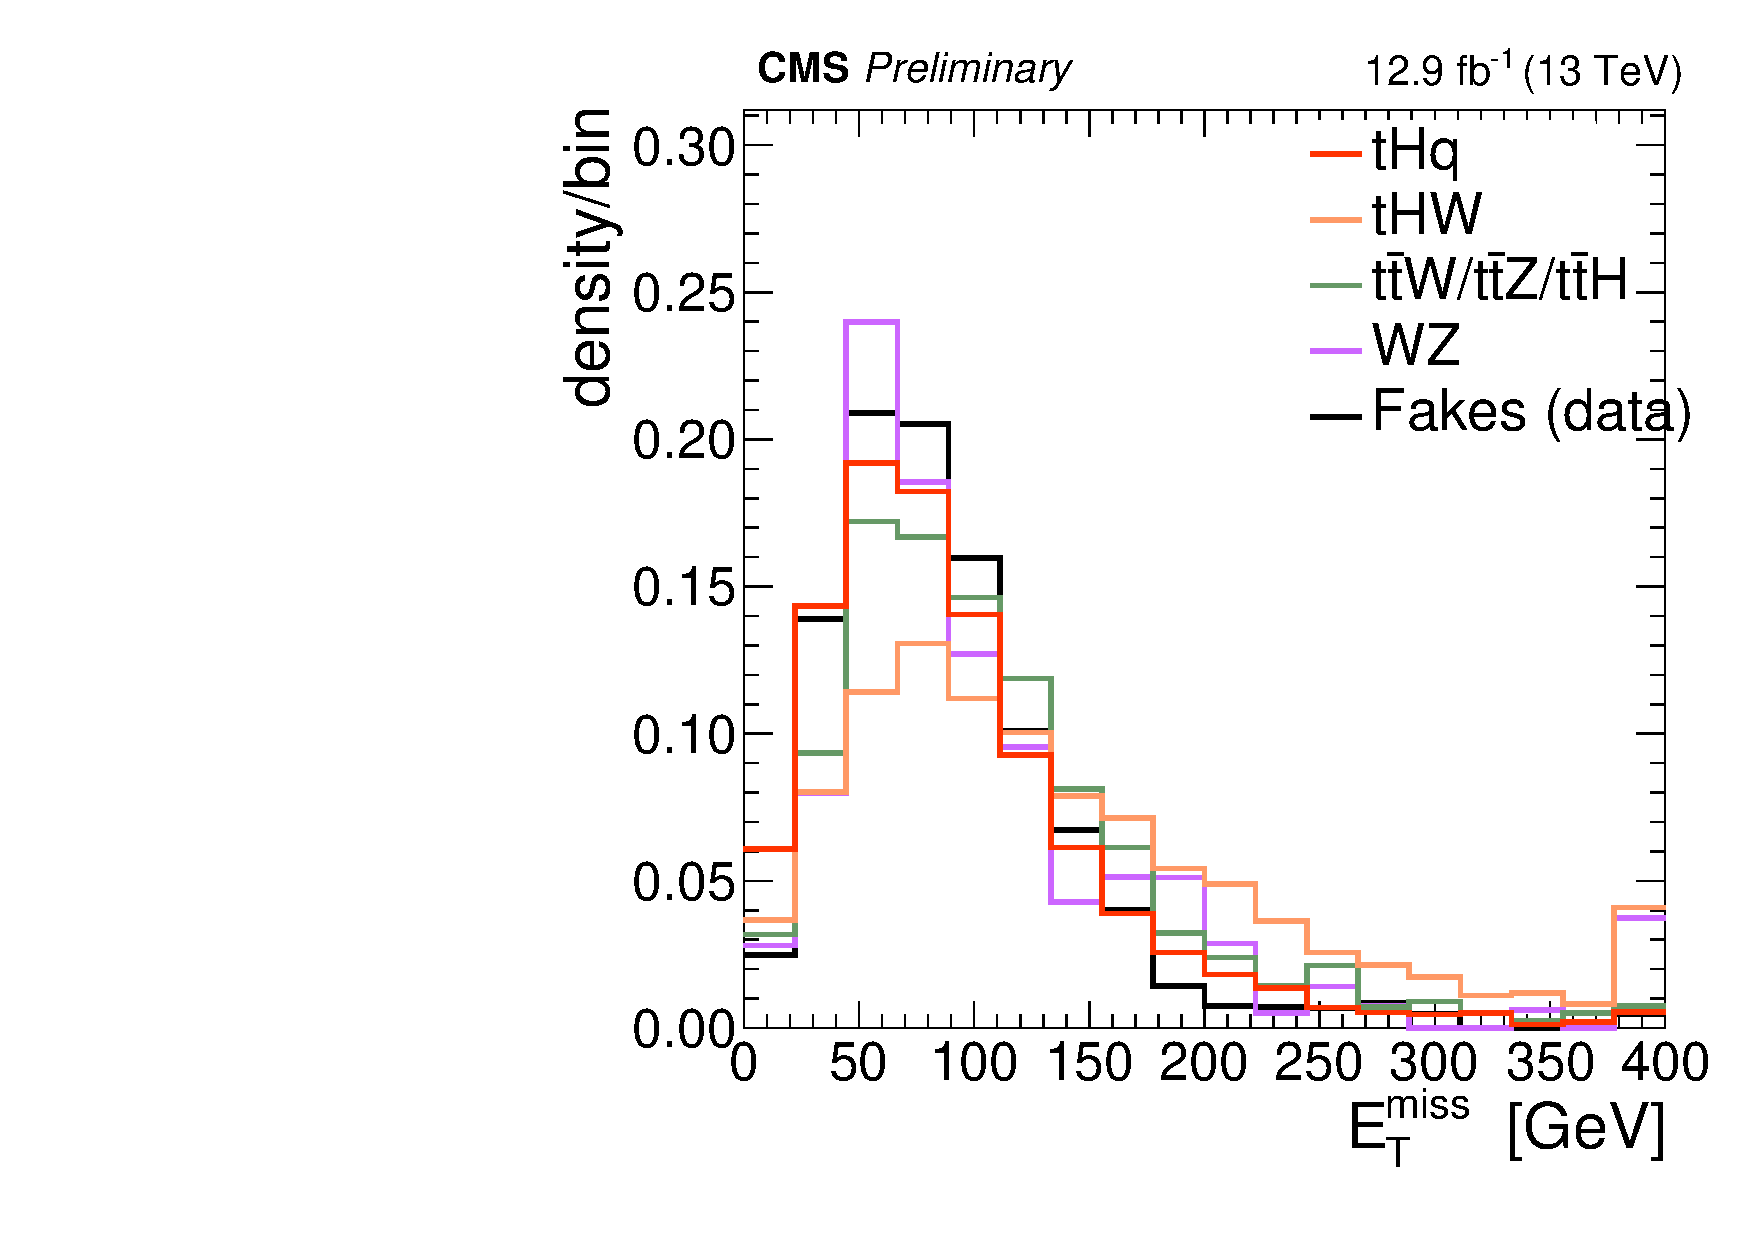
\includegraphics[width=0.30\textwidth]{figures/controlplots/3l-ttbar/met.pdf}
%   \includegraphics[width=0.30\textwidth]{figures/controlplots/3l-ttbar/nBJetLoose25.pdf}
%   \includegraphics[width=0.30\textwidth]{figures/controlplots/3l-ttbar/nJet25.pdf} 
% \caption{Kinematic distributions in the part of the signal region without a light forward jet ($max(\eta)<2$) to the three-lepton signal region.}
% \label{fig:3lttcontrol}
% \end{figure}

\subsection{Opposite-sign $\Pe\Pgm$ control region}\label{app:fwdcontrol}
We select a sample of dileptonic \ttbar\ events by requiring two opposite-sign tight leptons in the $\Pe\Pgm$ channel, with at least two jets and at least one medium CSV tagged jet. (Otherwise the selection is identical to the same-sign \emu\ channel selection.)
We study some distribution related to the forward jet modeling and compare the observed data with the predictions from \ttbar\ MC, see Fig.~\ref{fig:osemu-ttbar}.
The agreement of the $\eta$ distribution of forward jets for a \pt\ cut of 25\GeV\ is poor, especially at higher values of $|\eta|$.
The (central) jet multiplicity is poorly modeled by the MadgraphMLM sample used here; consistent with other observations of the same sample.
Note that the \ttbar\ background in this analysis is modeled with a data-driven method and these disagreements do not directly affect the \ttbar\ contribution in the analysis.
They do however reflect the expected agreement in these distributions for the irreducible backgrounds and the signal.
\begin{figure} [!h]
  \centering
  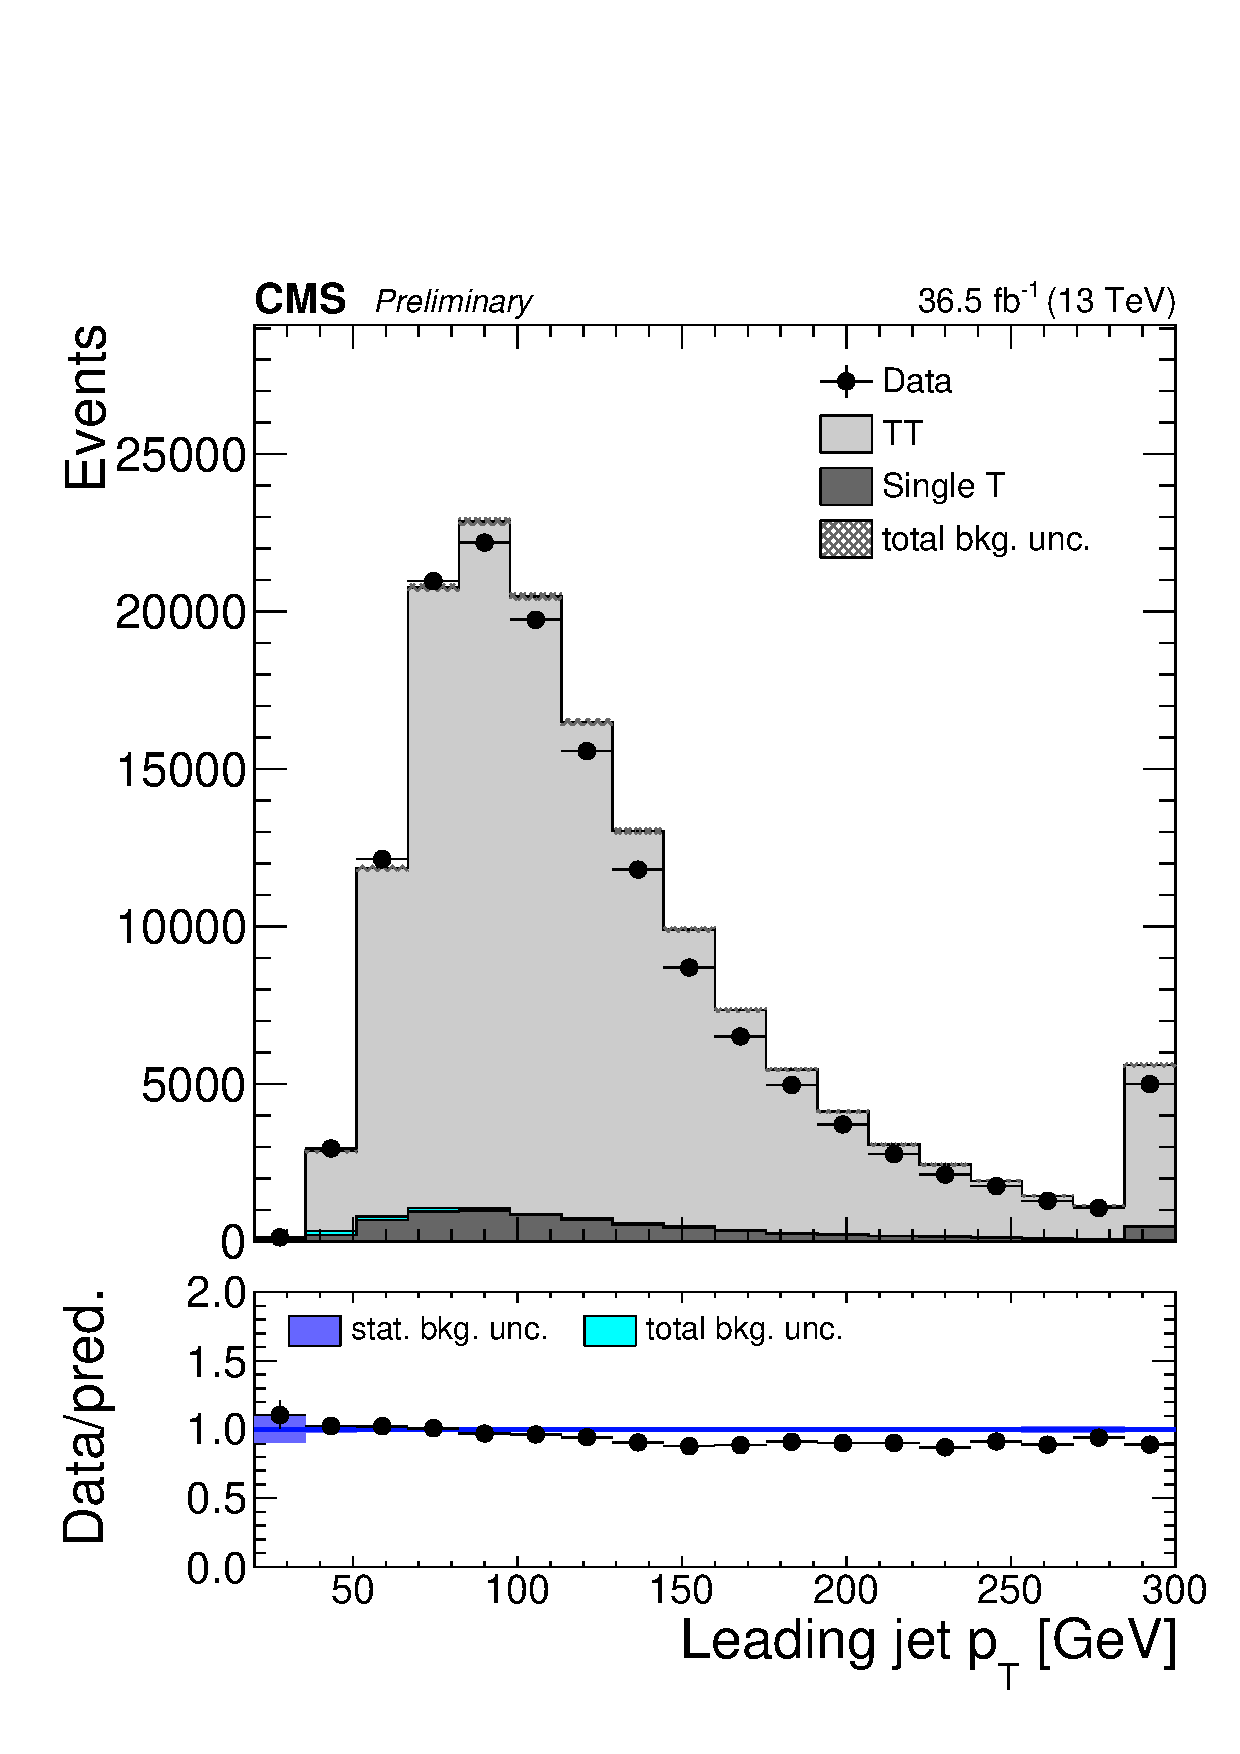
\includegraphics[width=0.30\textwidth]{figures/controlplots/emu-ttbar/Jet1pt.pdf}
  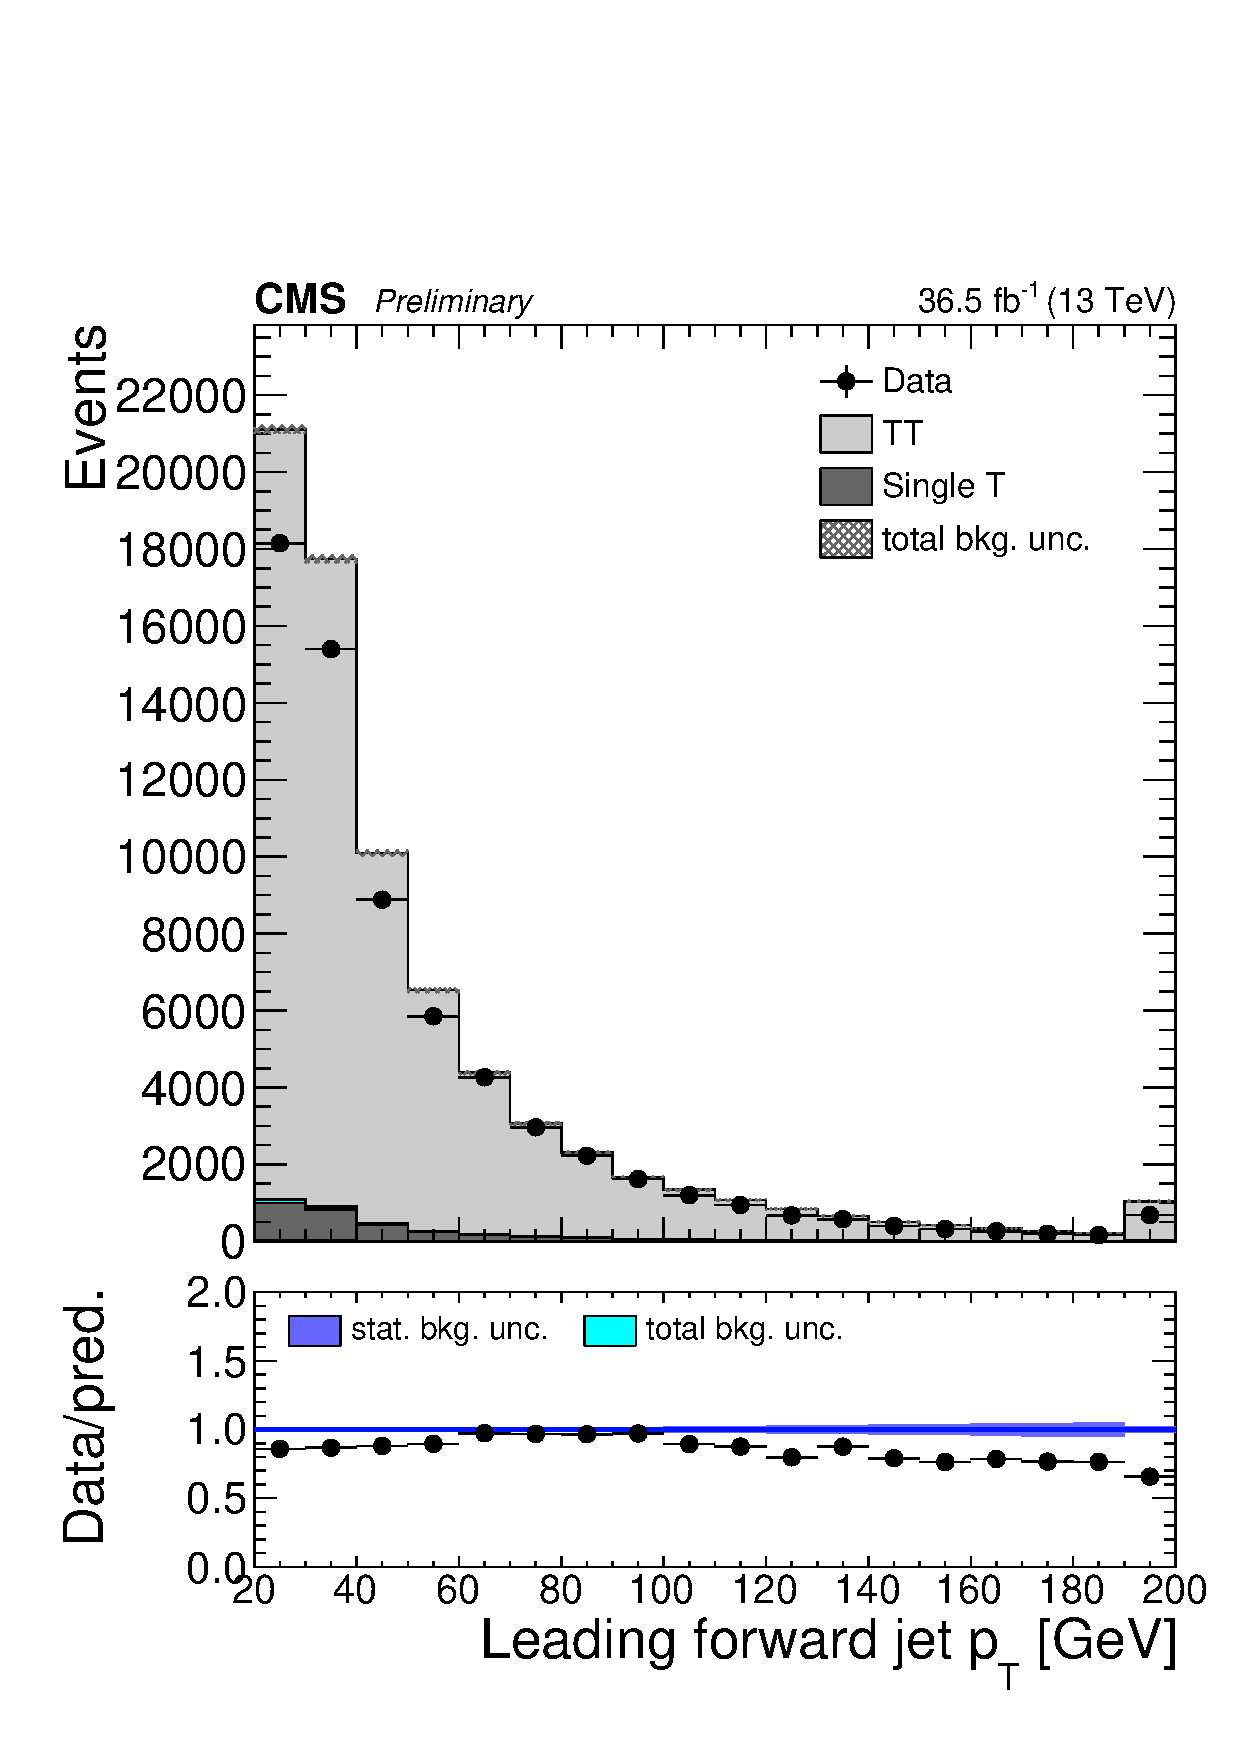
\includegraphics[width=0.30\textwidth]{figures/controlplots/emu-ttbar/JetFwd1pt.pdf}
  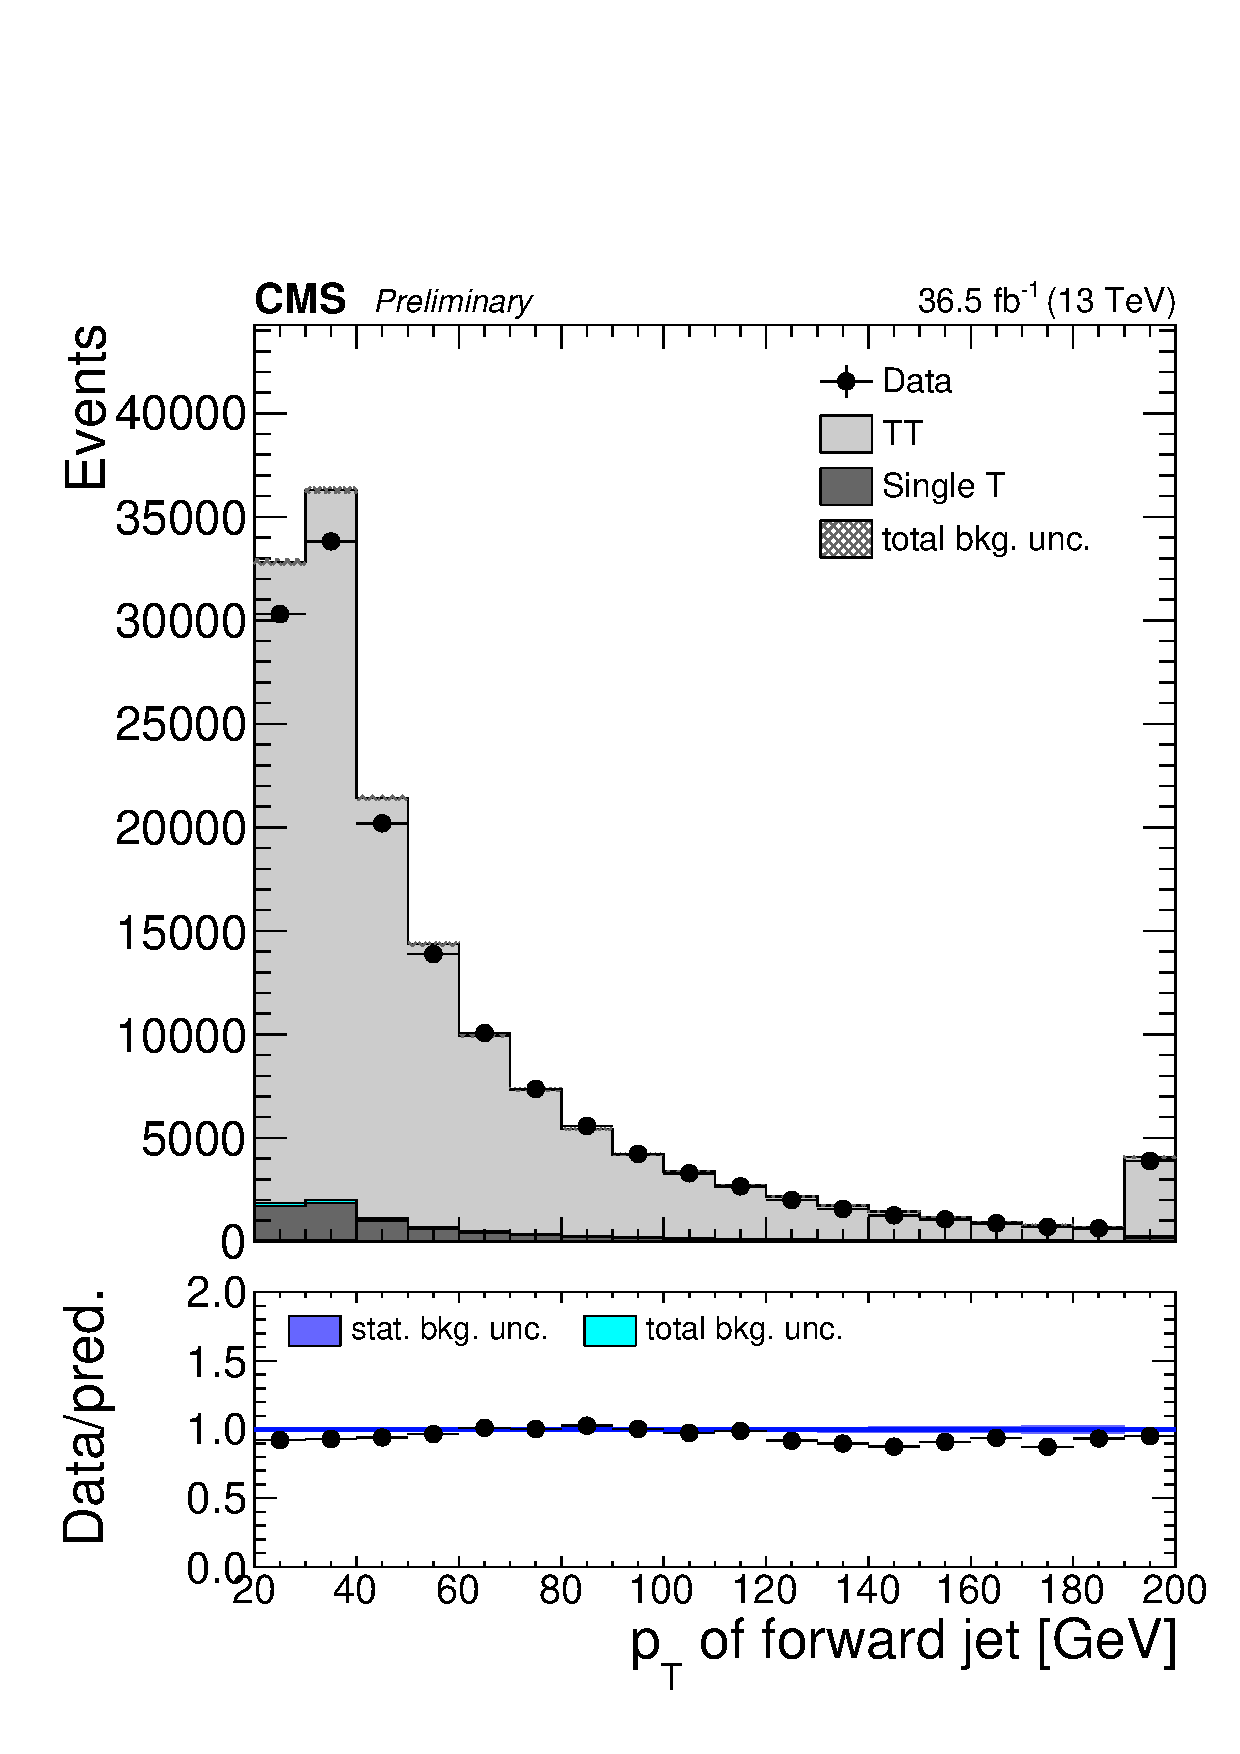
\includegraphics[width=0.30\textwidth]{figures/controlplots/emu-ttbar/fwdJetPt25.pdf} \\
  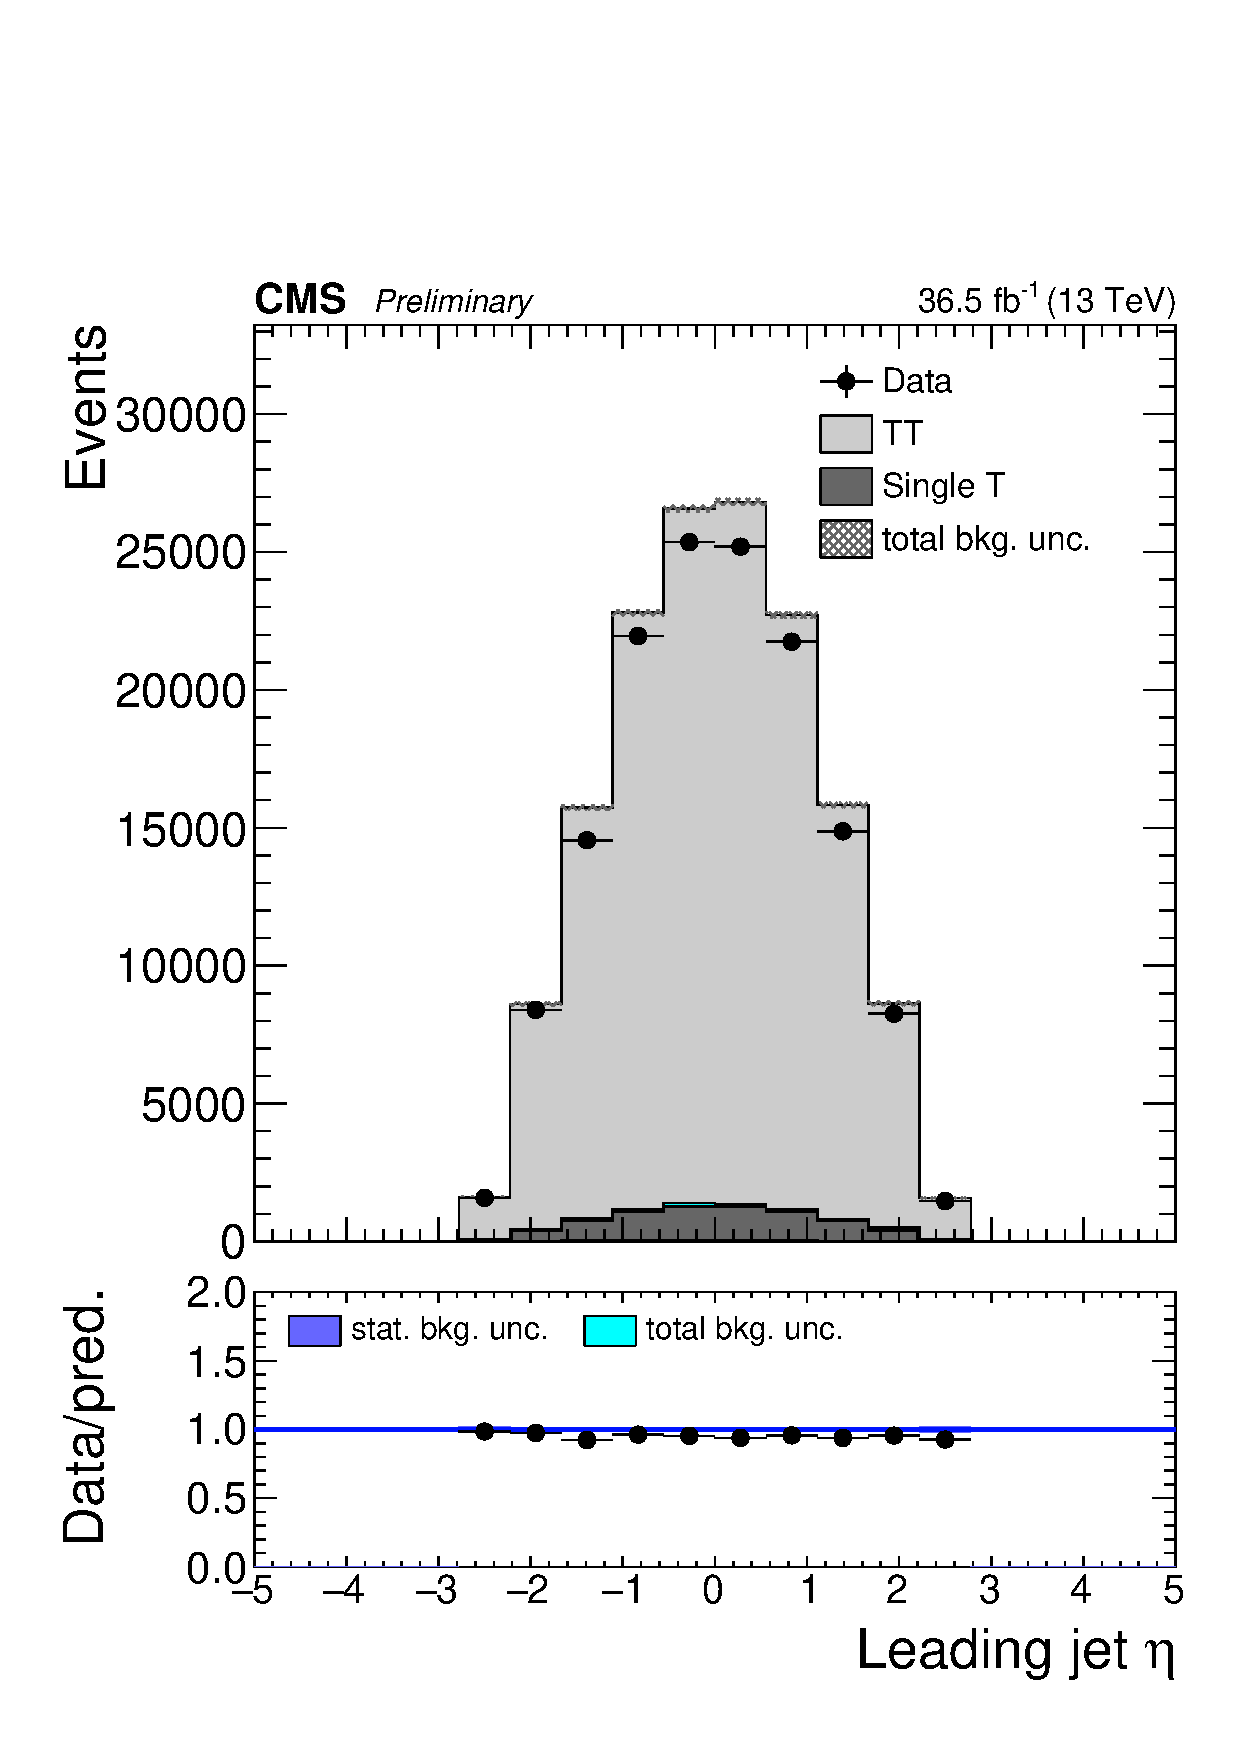
\includegraphics[width=0.30\textwidth]{figures/controlplots/emu-ttbar/Jet1eta.pdf}
  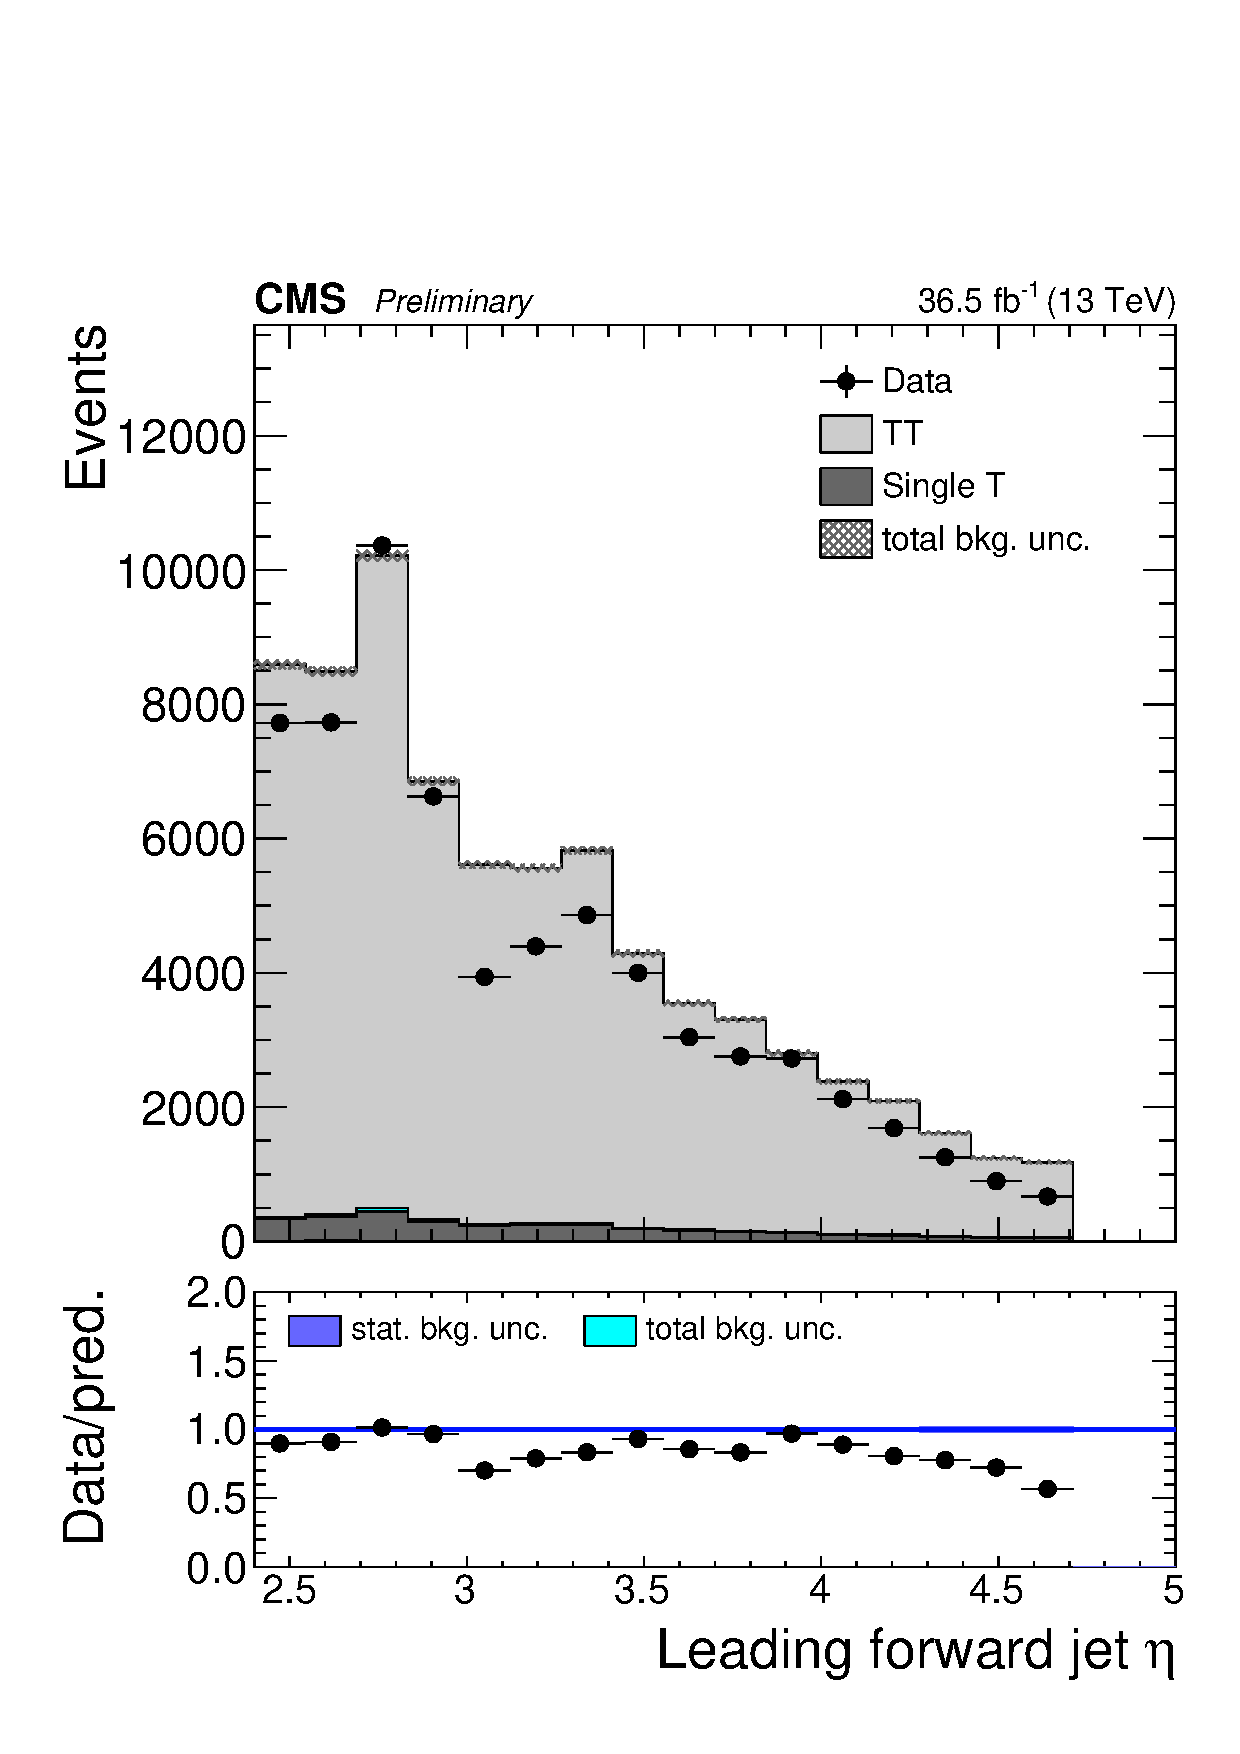
\includegraphics[width=0.30\textwidth]{figures/controlplots/emu-ttbar/JetFwd1eta.pdf}
  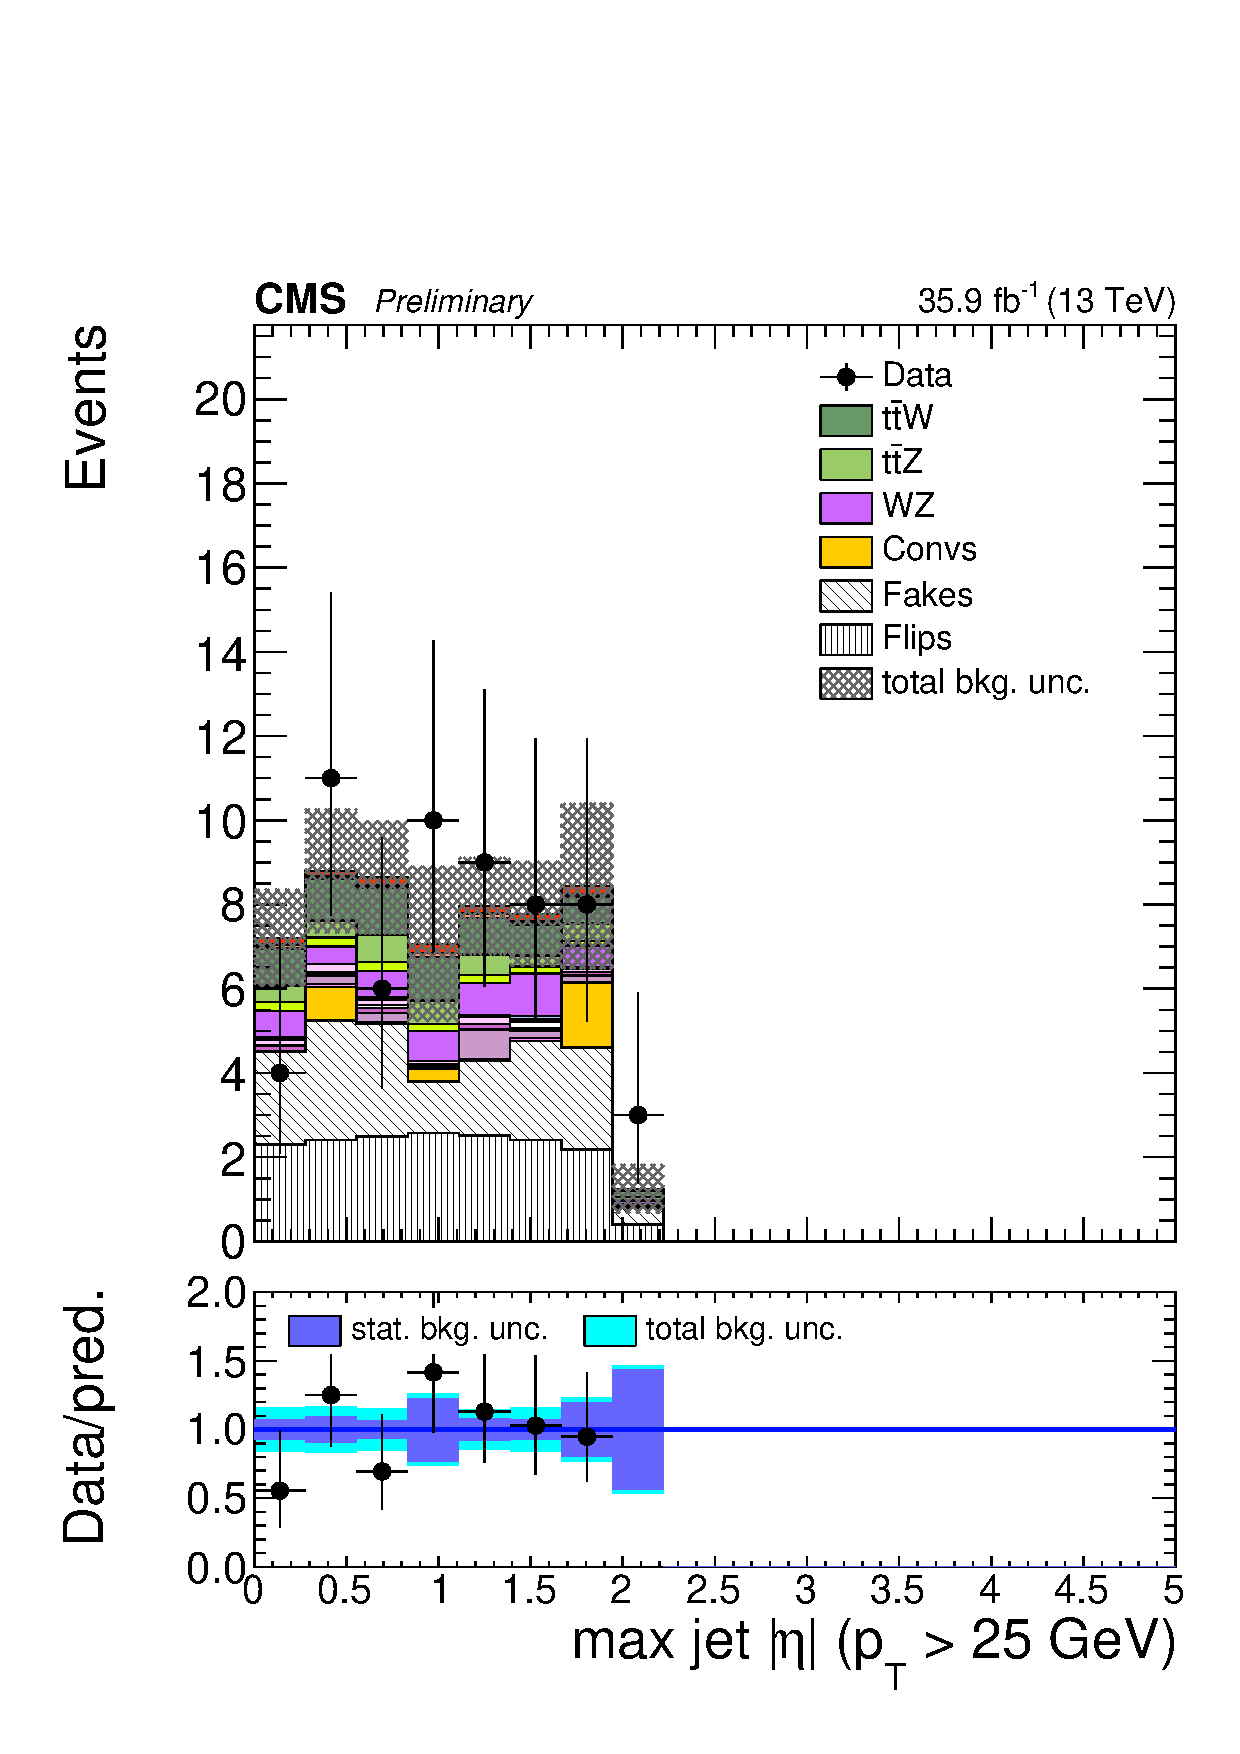
\includegraphics[width=0.30\textwidth]{figures/controlplots/emu-ttbar/maxEtaJet25.pdf} \\
  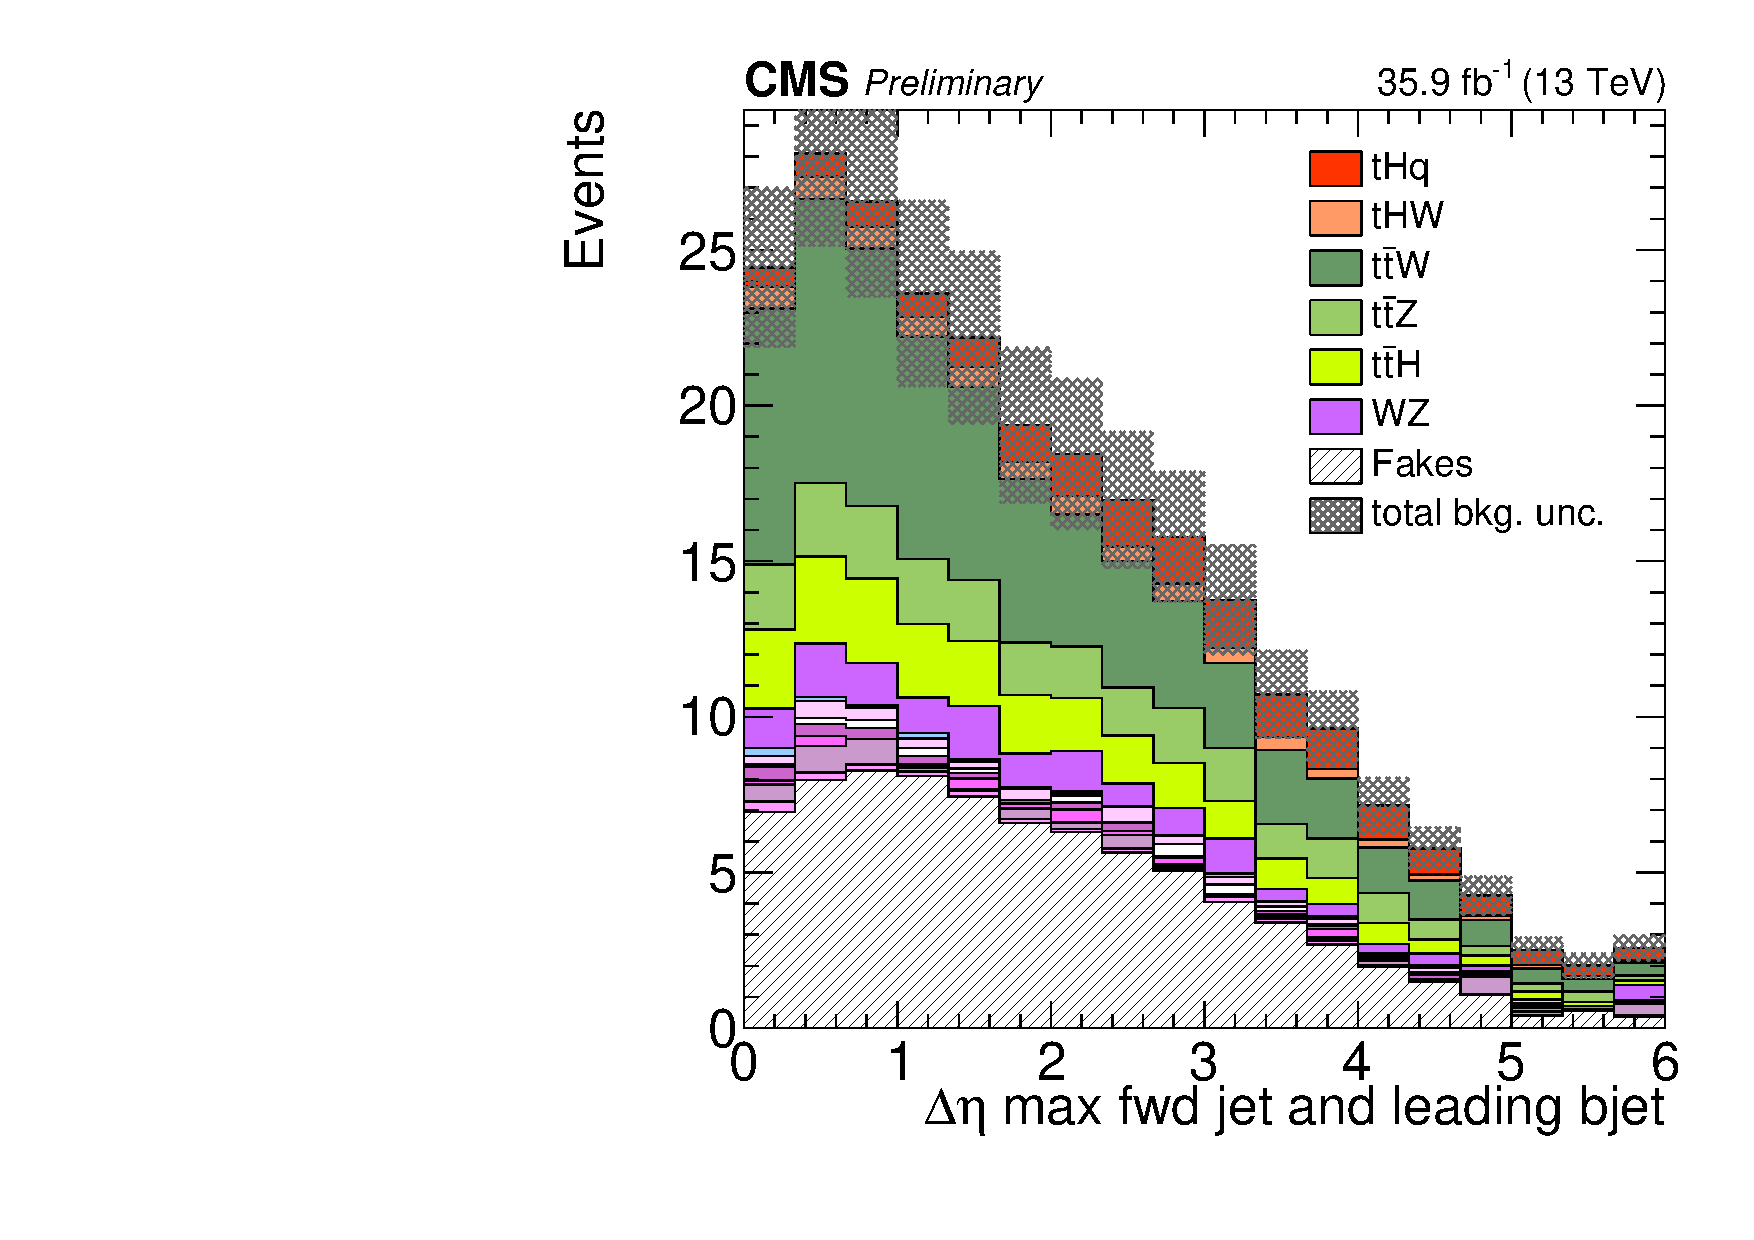
\includegraphics[width=0.30\textwidth]{figures/controlplots/emu-ttbar/dEtaFwdJetBJet.pdf}
  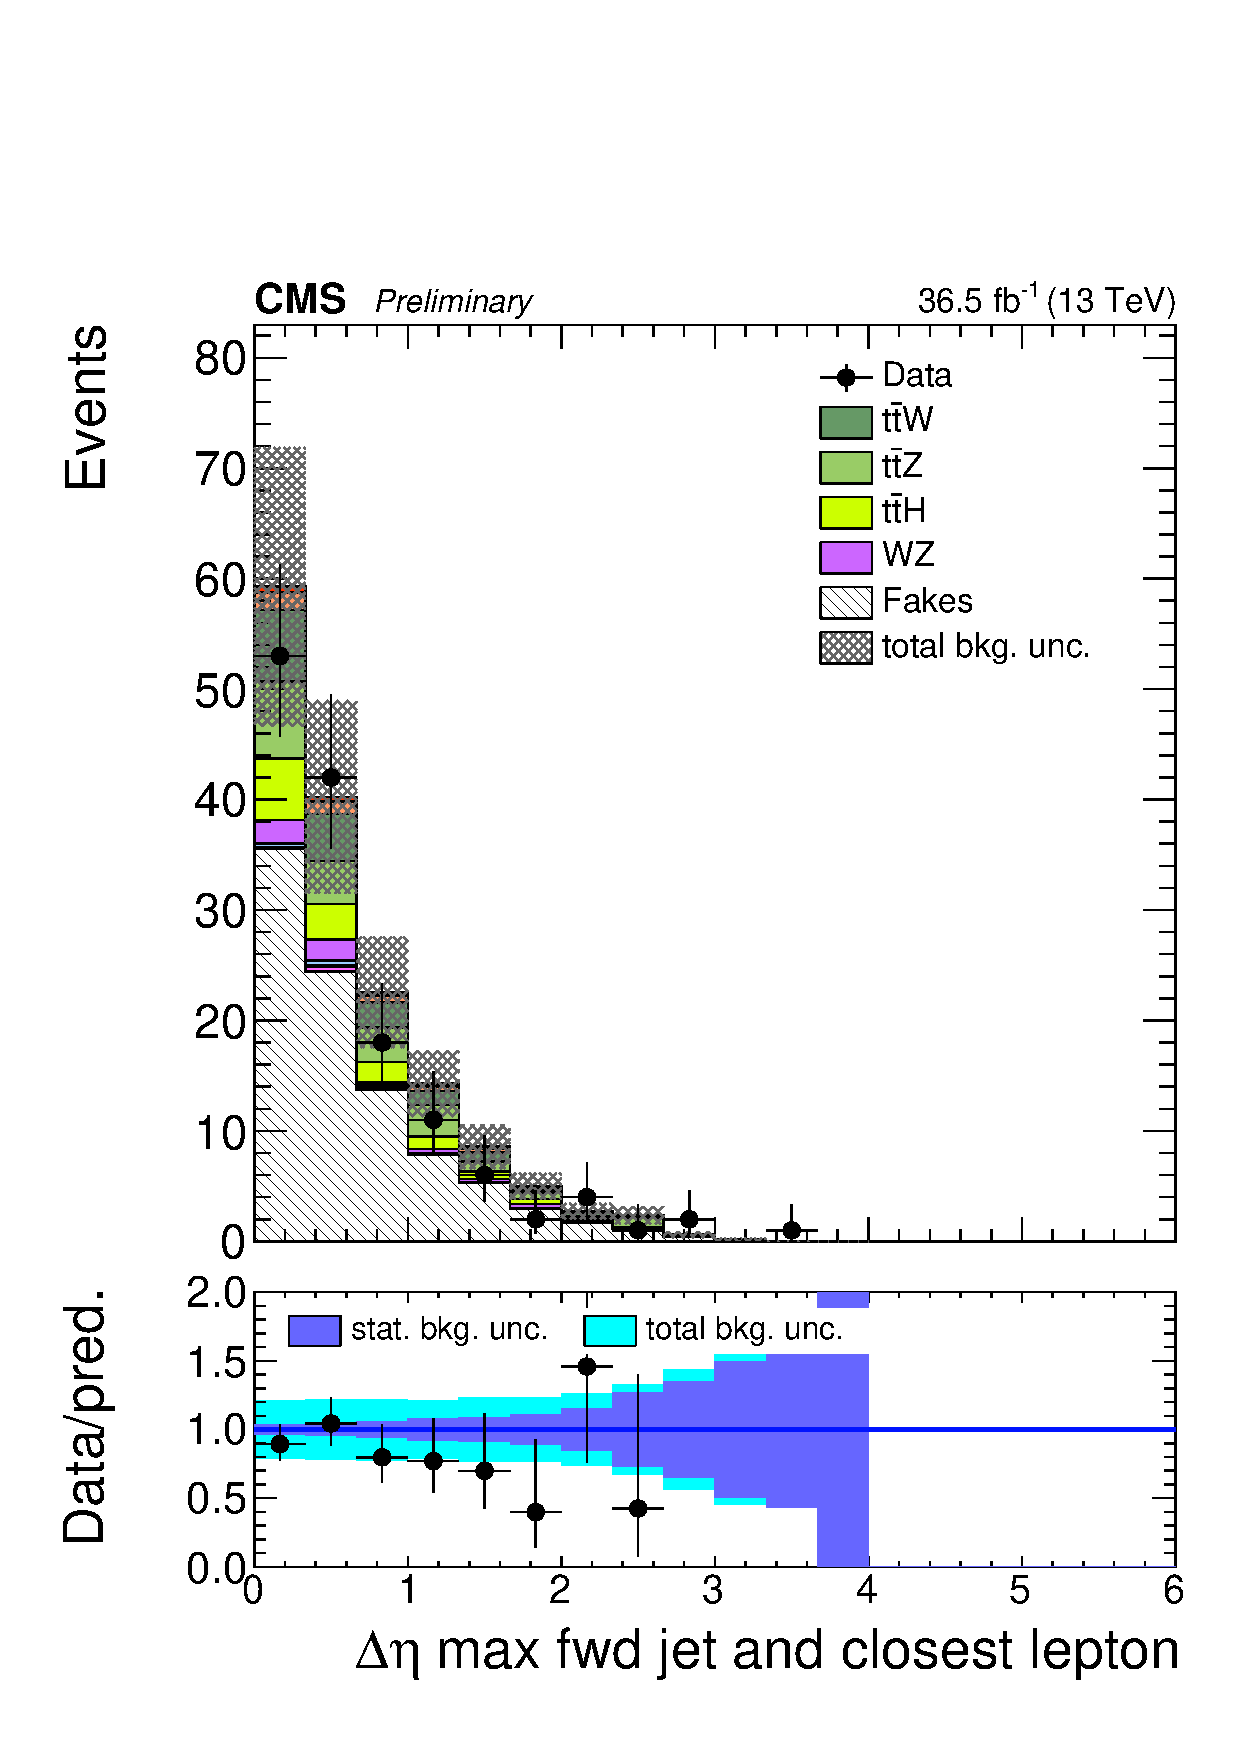
\includegraphics[width=0.30\textwidth]{figures/controlplots/emu-ttbar/dEtaFwdJetClosestLep.pdf}
  \includegraphics[width=0.30\textwidth]{figures/controlplots/emu-ttbar/nJet25.pdf} \\
\caption{Kinematic distributions in the \ttbar-enriched opposite-sign $\Pe\Pgm$ selection. Top row, left to right: leading central ($\eta<2.4$) jet \pt, leading forward ($\eta>2.4$) jet \pt, \pt\ of non-CSV-loose jet with highest $\eta$ (``light forward jet''). Middle row: $\eta$ distribution of those same jets. Bottom row: $\Delta\eta$ between light forward jet and leading CSV-loose tagged jet; $\Delta\eta$ between light forward jet and closest lepton; number of central jets.}
\label{fig:osemu-ttbar}
\end{figure}

The data/MC agreement in the forward jet $\eta$ distribution improves significantly at higher jet $\pt$s.
% Figure~\ref{fig:osemu-fwdjet} shows the agreement for \pt\ cuts of $25\GeV$ and $50\GeV$.
% \begin{figure} [!h]
%   \centering
%   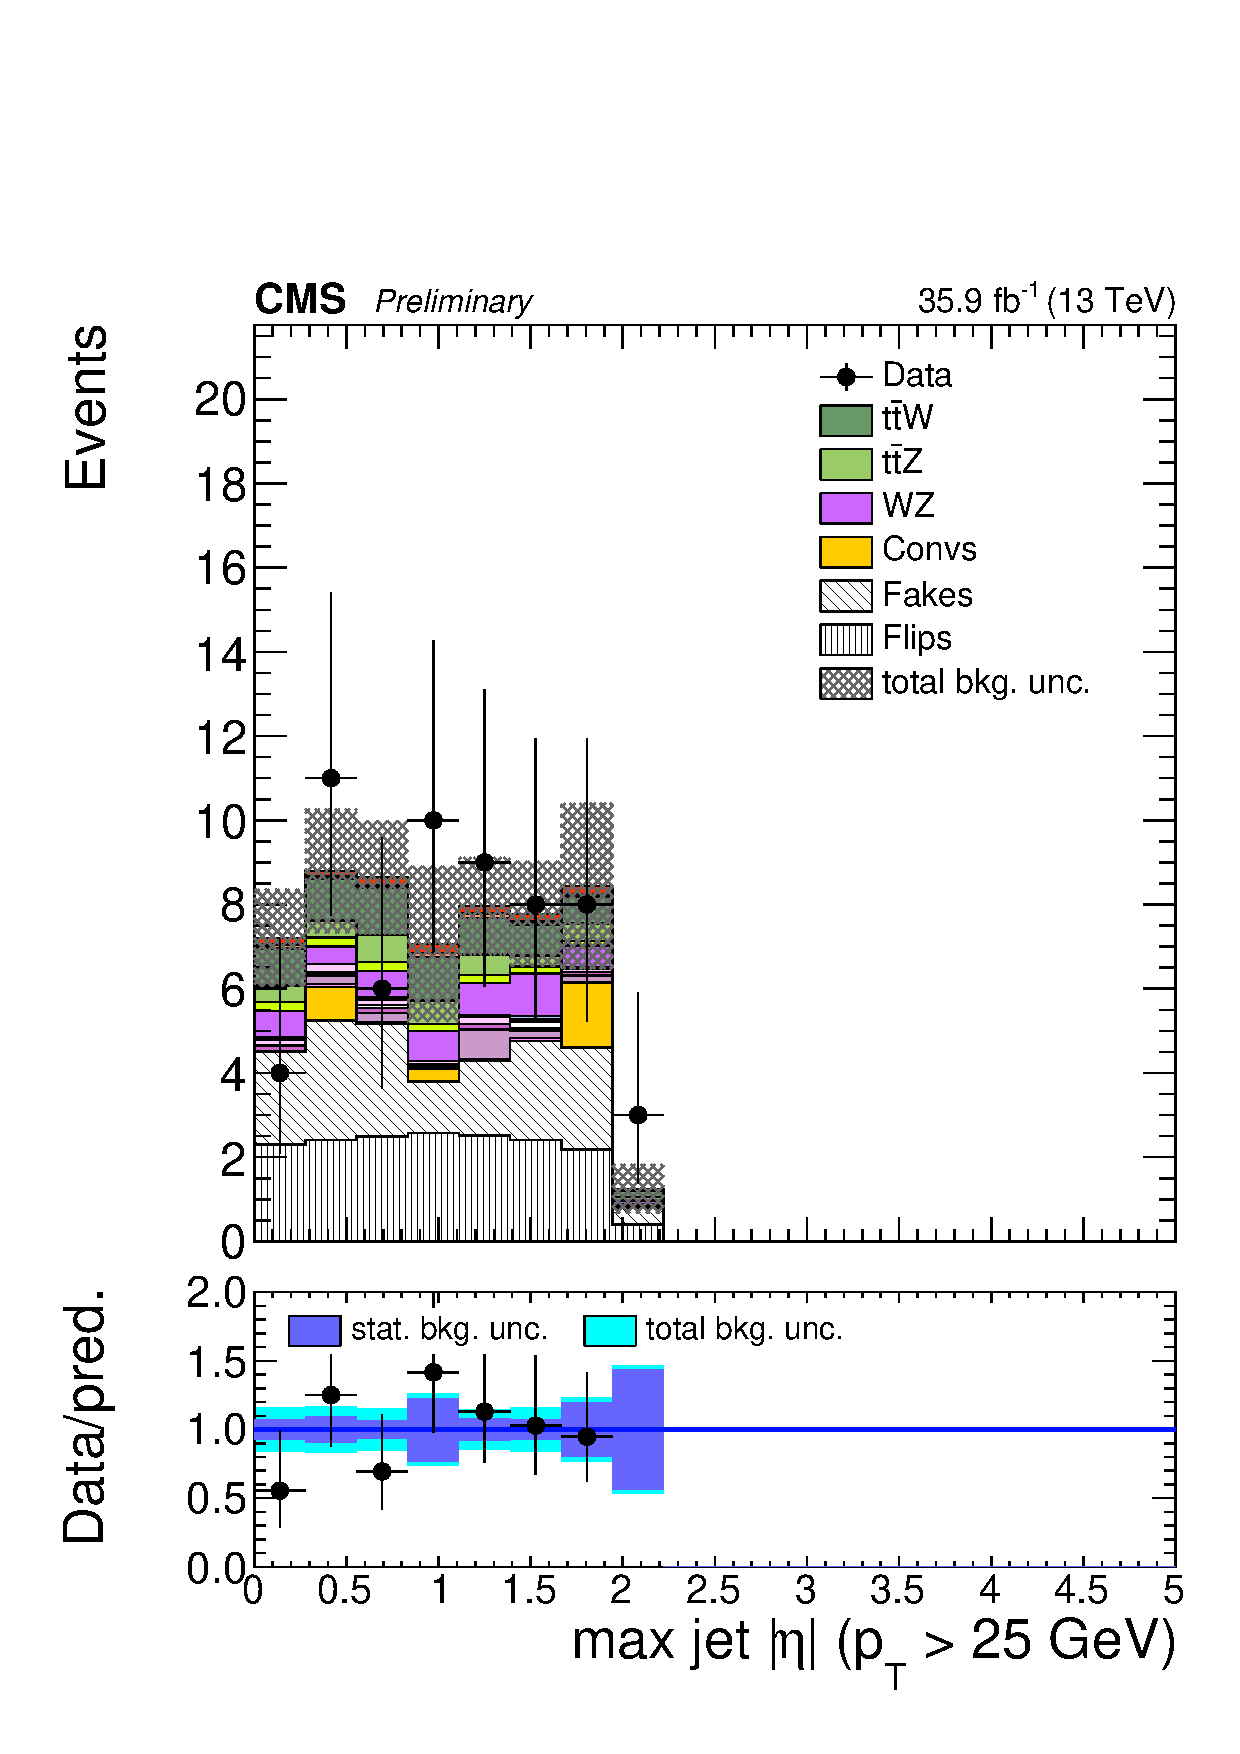
\includegraphics[width=0.40\textwidth]{figures/controlplots/emu-ttbar/maxEtaJet25.pdf}
%   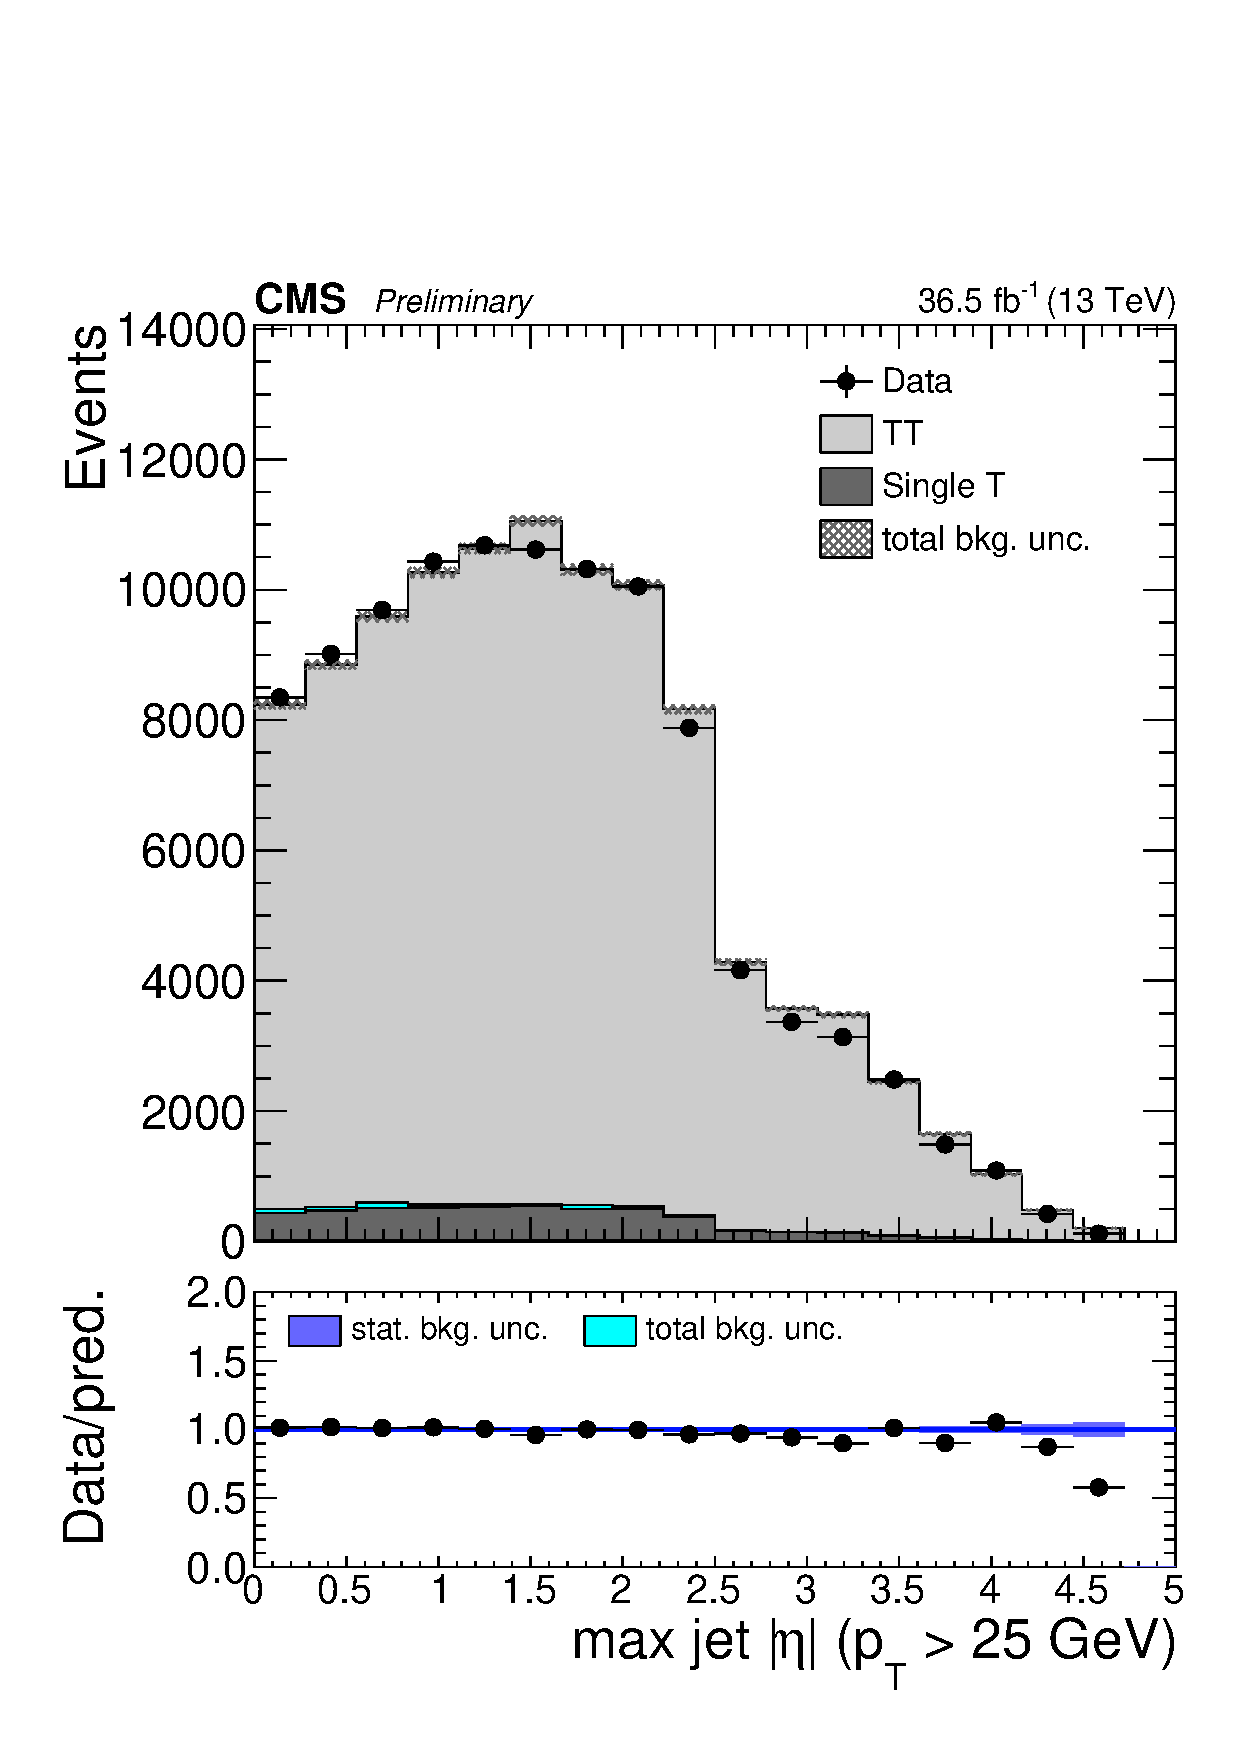
\includegraphics[width=0.40\textwidth]{figures/controlplots/emu-ttbar/maxEtaJet25_fwdjet50.pdf}
% \caption{Pseudorapidity distributions of the most forward, non-CSV-loose tagged jet in the \ttbar-enriched opposite-sign $\Pe\Pgm$ selection. Left for a \pt\ cut of $25\GeV$, right for $50\GeV$.}
% \label{fig:osemu-fwdjet}
% \end{figure}

The effect of higher $\pt$ cuts on the forward jet has been studied for three values: $25$, $30$ and $40\GeV$.
In order to take into account the data/MC disagreement in the high $\eta$ regions, the events are weighted accordingly to the data/MC ratio of the unity normalized control plots shown in Fig.~\ref{fig:ptCutVar}.
\begin{figure} [!h]
  \centering
  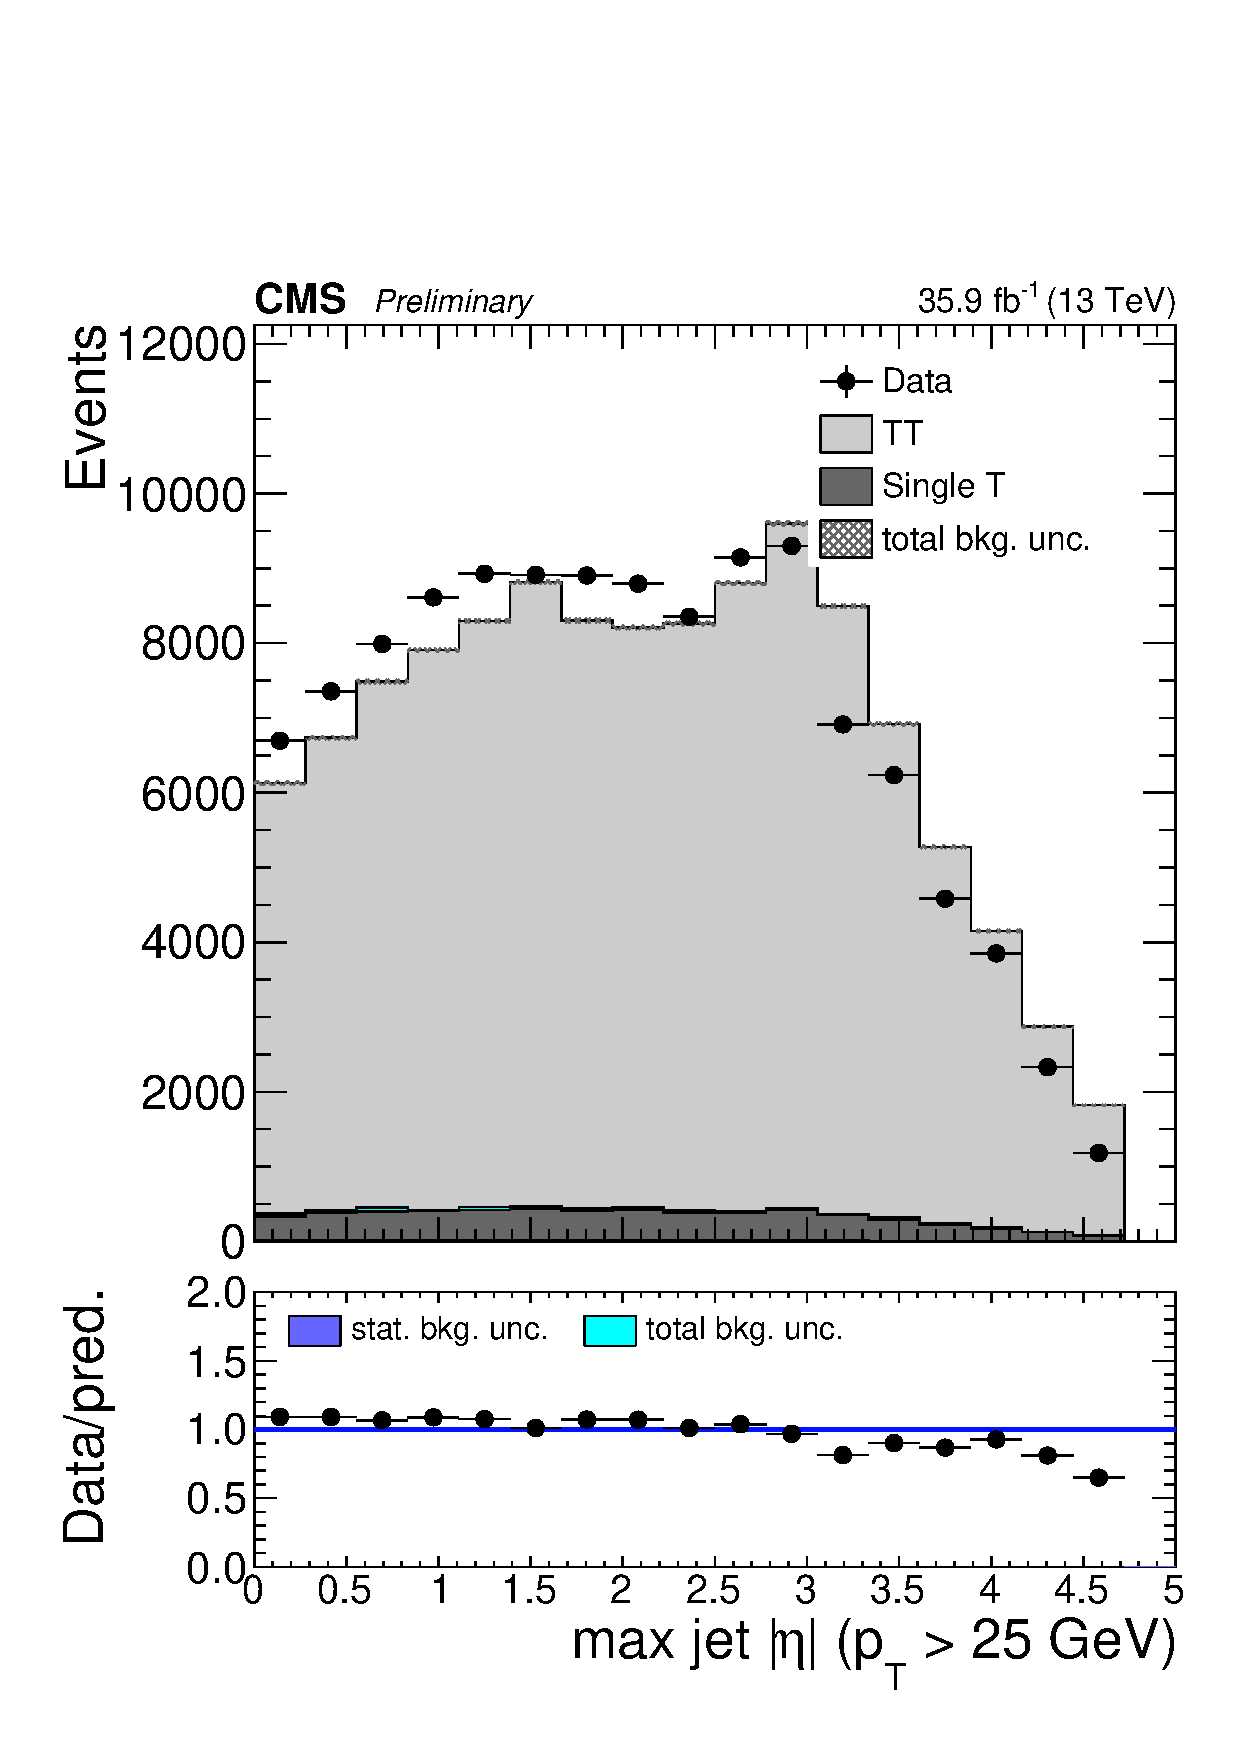
\includegraphics[width=0.30\textwidth]{figures/controlplots/emu-ttbar/maxEtaJet25_25.pdf}
  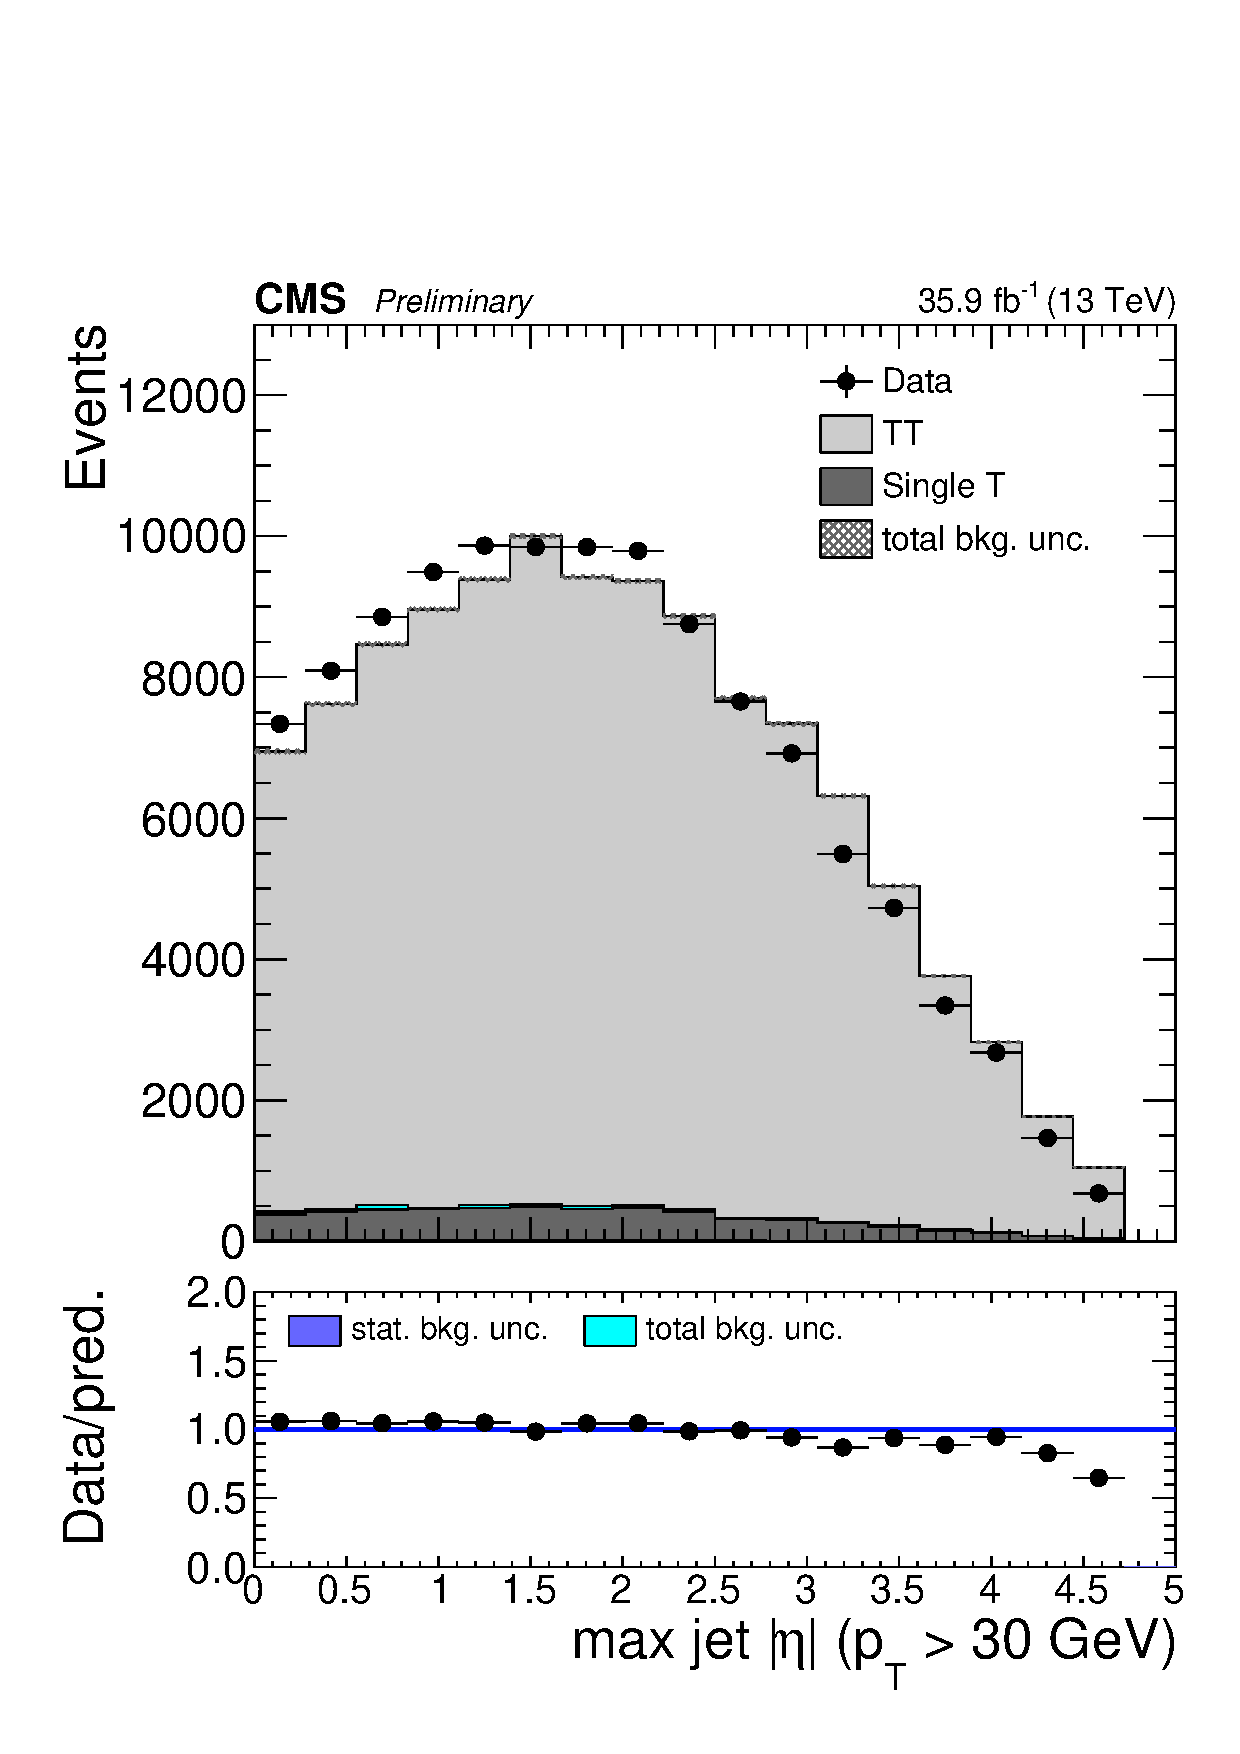
\includegraphics[width=0.30\textwidth]{figures/controlplots/emu-ttbar/maxEtaJet25_30.pdf}
  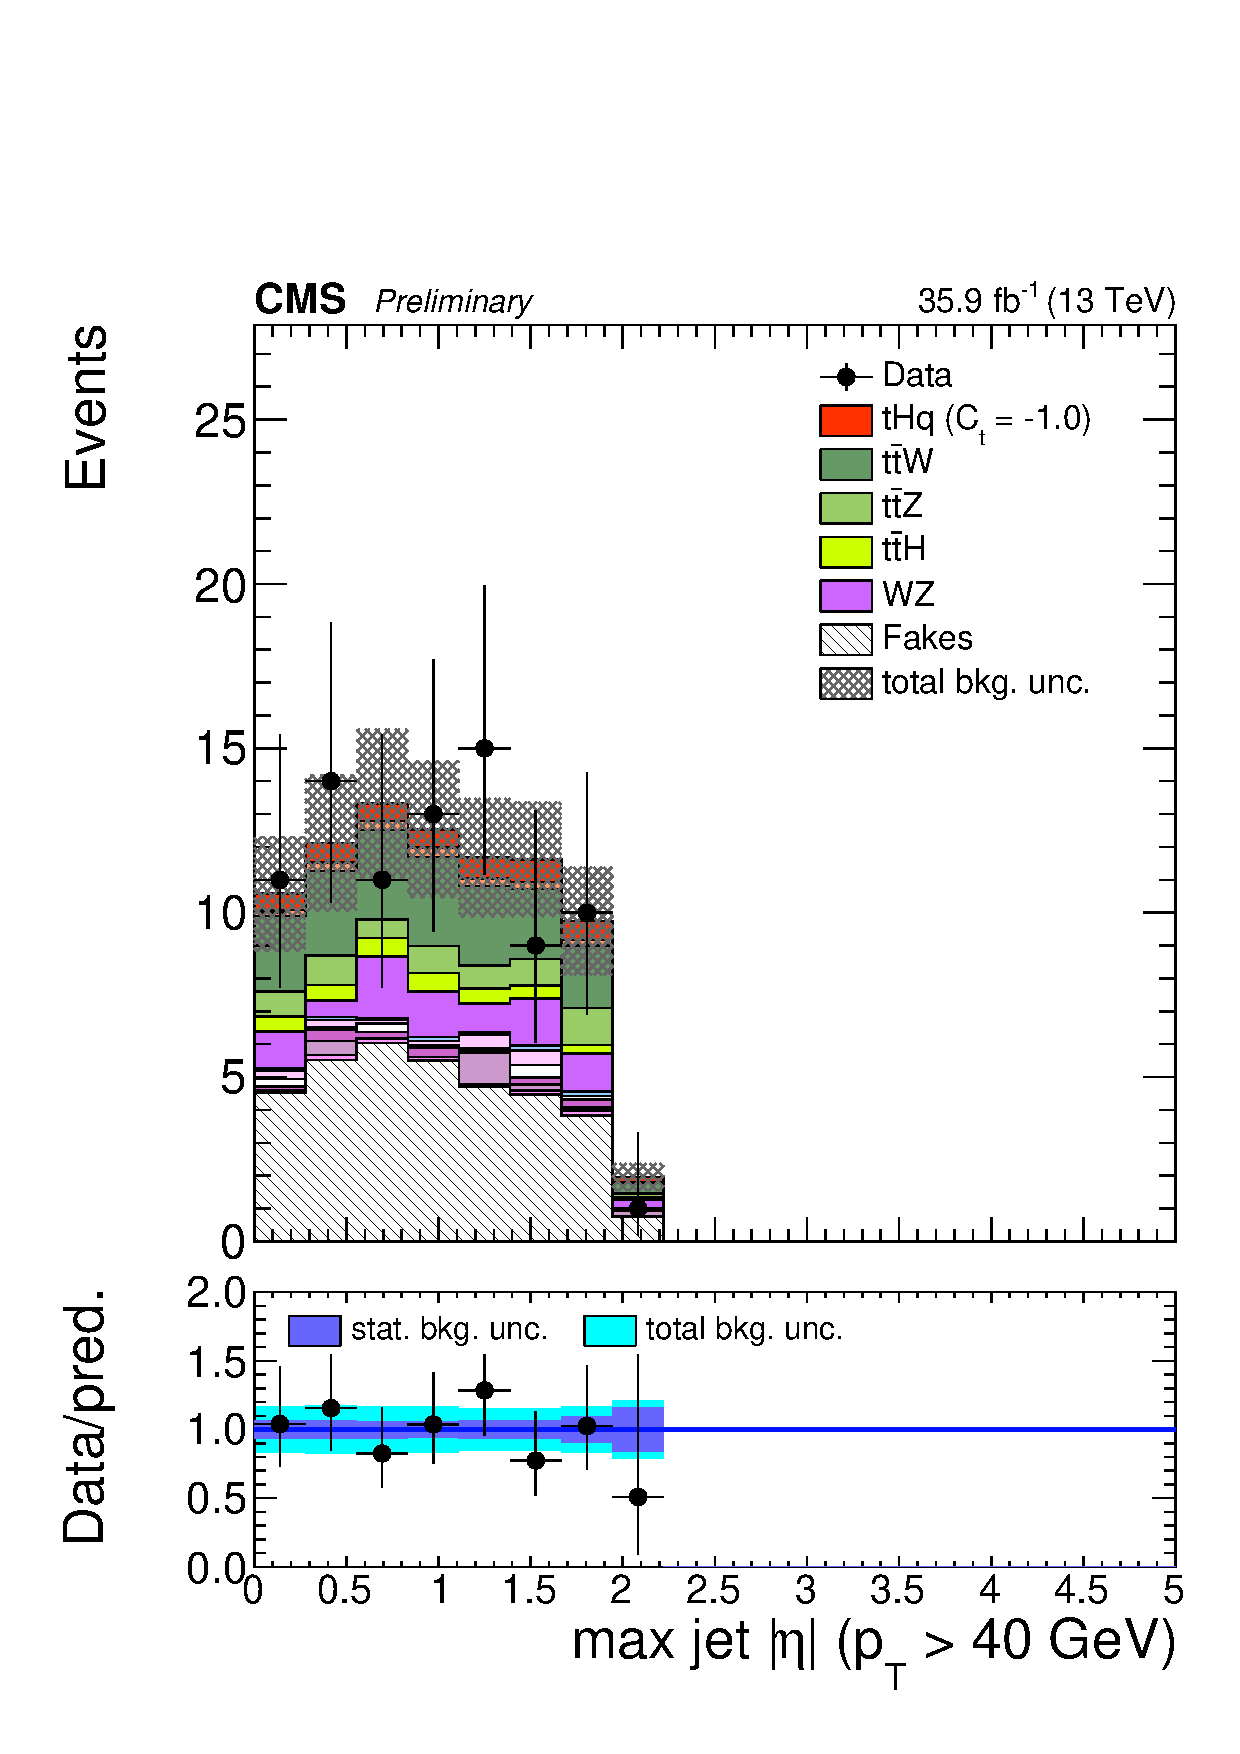
\includegraphics[width=0.30\textwidth]{figures/controlplots/emu-ttbar/maxEtaJet25_40.pdf}\\
\caption{Pseudorapidity distributions of the most forward, non-CSV-loose tagged jet in the tt-enriched opposite-sign $\Pe\Pgm$ selection for the three $\pt$ cut values.}
\label{fig:ptCutVar}
\end{figure}

Table~\ref{tab:ratioFwdJet} shows the scale factors obtained for the three $\pt$ values.
\begin{table}[thb]
\centering
\begin{tabular}{lrrr}
\multicolumn{1}{c@{\qquad}}{$\eta$ range} &
\multicolumn{1}{c}{$\pt>25\GeV$} &
\multicolumn{1}{c}{$\pt>30\GeV$} & 
\multicolumn{1}{c}{$\pt>40\GeV$}\\ \hline
$0-0.278$     & $1.0925$ & $1.0566$ & $1.0326$ \\
$0.278-0.556$ & $1.0920$ & $1.0617$ & $1.0407$ \\ 
$0.556-0.833$ & $1.0675$ & $1.0459$ & $1.0244$ \\
$0.833-1.111$ & $1.0888$ & $1.0593$ & $1.0340$ \\
$1.111-1.389$ & $1.0759$ & $1.0508$ & $1.0322$ \\
$1.389-1.667$ & $1.0109$ & $0.9847$ & $0.9661$ \\
$1.667-1.944$ & $1.0727$ & $1.0448$ & $1.0239$ \\
$1.944-2.222$ & $1.0715$ & $1.0457$ & $1.0169$ \\
$2.222-2.500$ & $1.0112$ & $0.9871$ & $0.9746$ \\
$2.500-2.778$ & $1.0387$ & $0.9942$ & $0.9816$ \\
$2.778-3.056$ & $0.9687$ & $0.9427$ & $0.9200$ \\
$3.056-3.333$ & $0.8137$ & $0.8695$ & $0.9092$ \\
$3.333-3.611$ & $0.9010$ & $0.9387$ & $0.9807$ \\
$3.611-3.889$ & $0.8685$ & $0.8887$ & $0.9213$ \\
$3.889-4.167$ & $0.9277$ & $0.9466$ & $1.0135$ \\
$4.167-4.444$ & $0.8111$ & $0.8278$ & $0.8637$ \\
$4.444-4.722$ & $0.6497$ & $0.6485$ & $0.6367$ \\
$4.722-5.000$ & $1.0000$ & $1.0000$ & $1.0000$ \\ \hline
Exp.\ limit (\threel) & $r<1.54$ & $r<1.51$ & $r<1.50$ \\ \hline
\end{tabular}
\caption{Data/MC scale factors for $\eta$ distribution of most forward, non-tagged jet with three different $\pt$ cuts, see Fig.~\ref{fig:ptCutVar}.}
\label{tab:ratioFwdJet}
\end{table}

With higher cuts in $\pt$, the expected limit on cross section in the three lepton channel improves from $1.54$ at $25\GeV$ to $1.51$ at $30\GeV$ and $1.50$ at $40\GeV$.
Adjusting the data/MC ratios by hand to half the obtained value in case of forward jet $\eta$ cut at $25$ GeV, improves the limit from $1.54$ to $1.51$ in the three lepton channel.
The impact of the data/MC disagreement for forward jet $\eta$ is observed to reduce with higher $\pt$ cuts.
Fig.~\ref{fig:impact25}, Fig.~\ref{fig:impact30} and Fig.~\ref{fig:impact40} show this reduction in the impact of the forward jet $\eta$ nuisance in the fit.

\begin{figure} [!h]
 \centering
 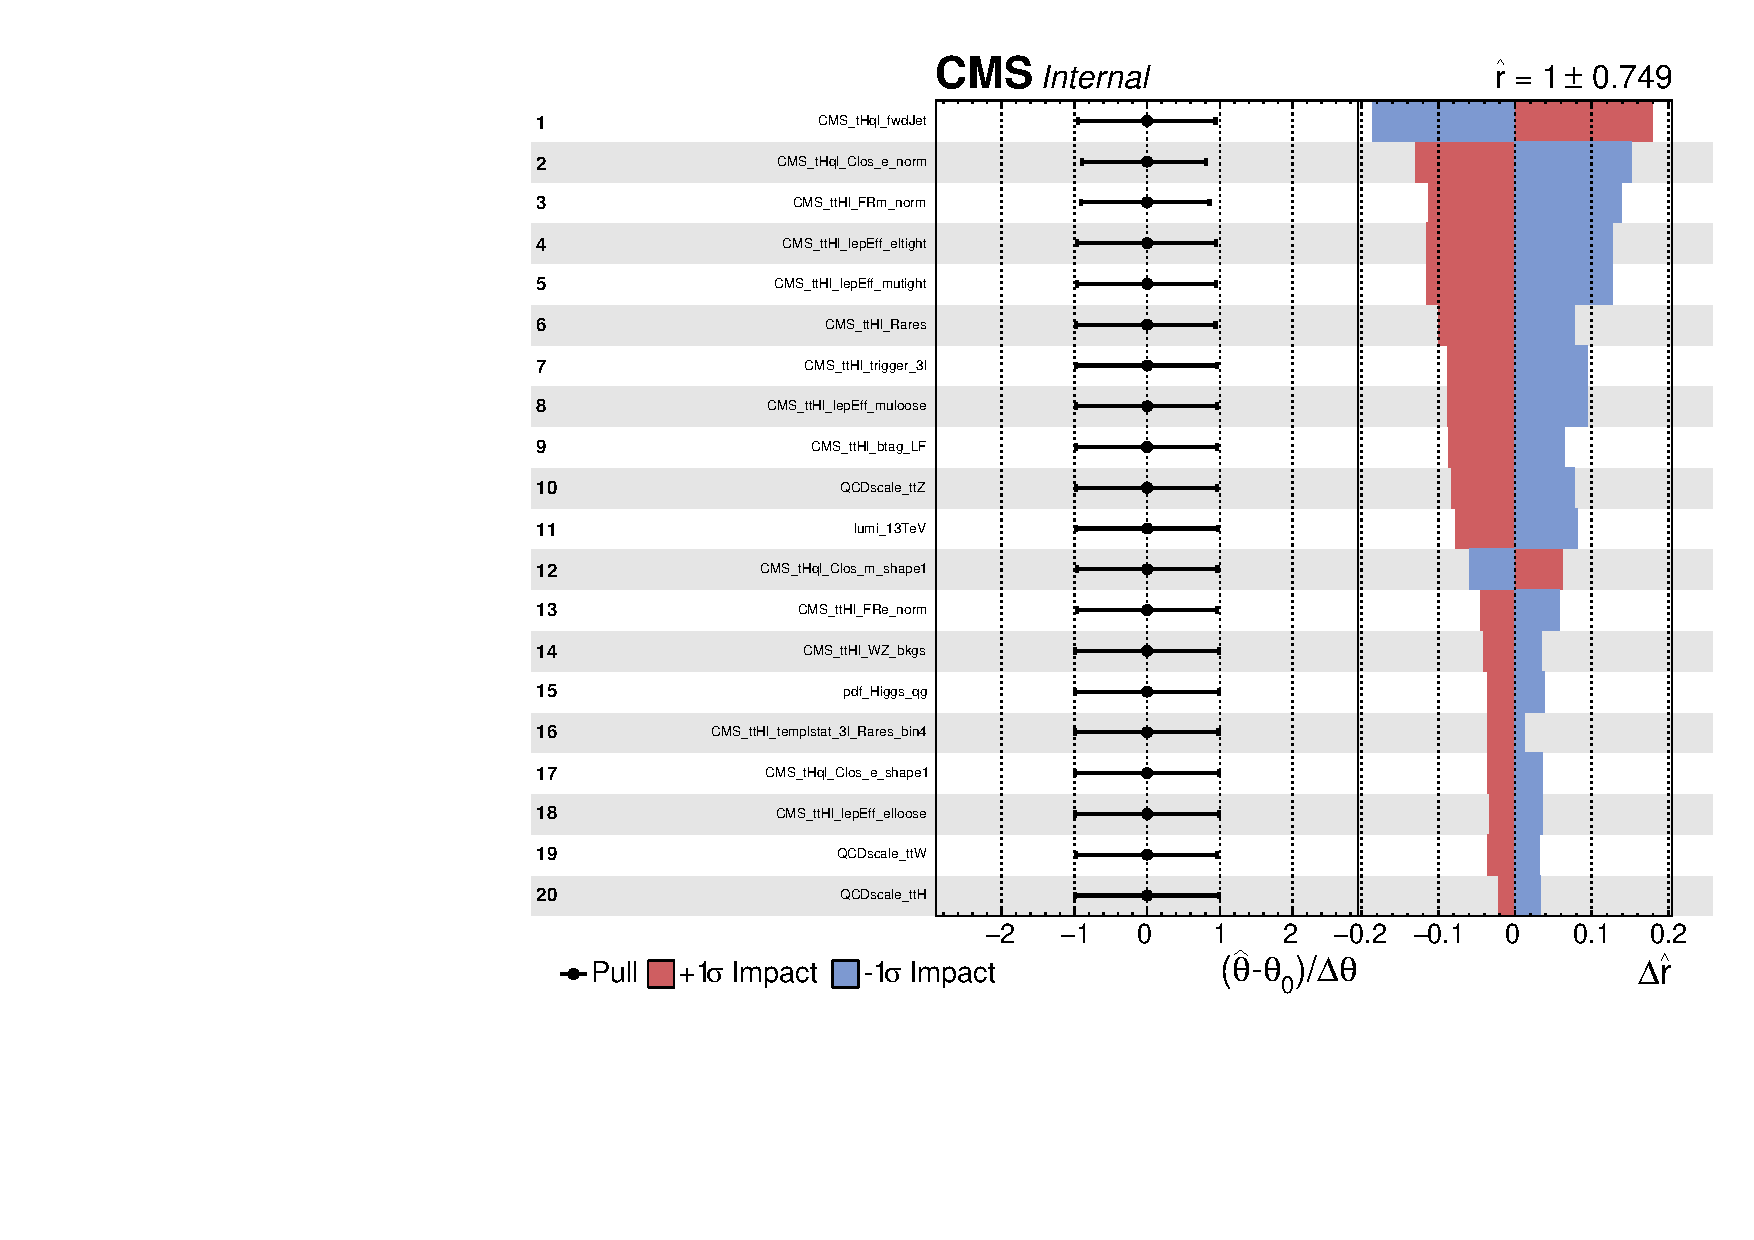
\includegraphics[width=1.0\textwidth]{figures/limits/impacts/impacts_25.pdf}\\
\caption{Post-fit pulls and impacts of the 20 nuisance parameters with $\pt$ cut $25$ GeV for the forward jet.}
\label{fig:impact25}
\end{figure}

\begin{figure} [!h]
 \centering
 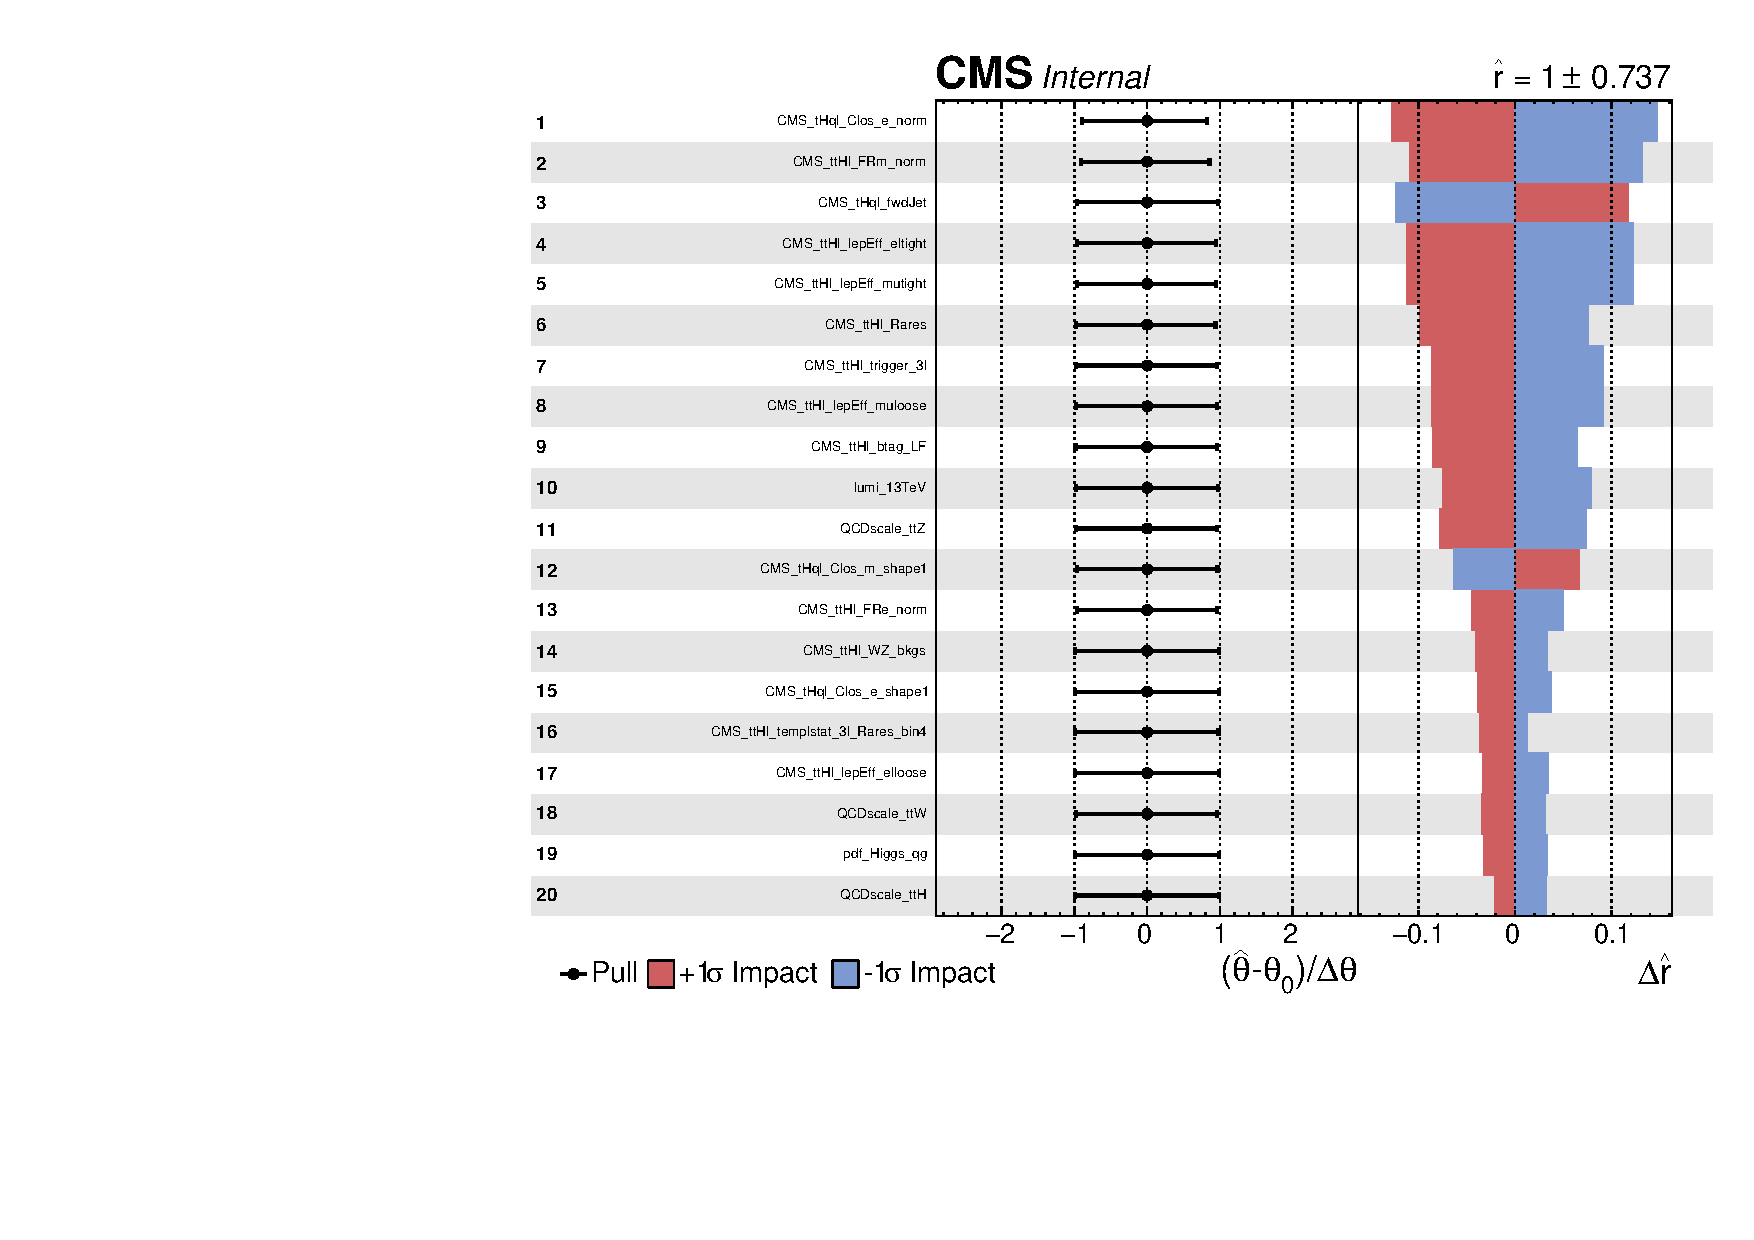
\includegraphics[width=1.0\textwidth]{figures/limits/impacts/impacts_30.pdf}\\
\caption{Post-fit pulls and impacts of the 20 nuisance parameters with $\pt$ cut $30$ GeV for the forward jet.}
\label{fig:impact30}
\end{figure}

\begin{figure} [!h]
 \centering
 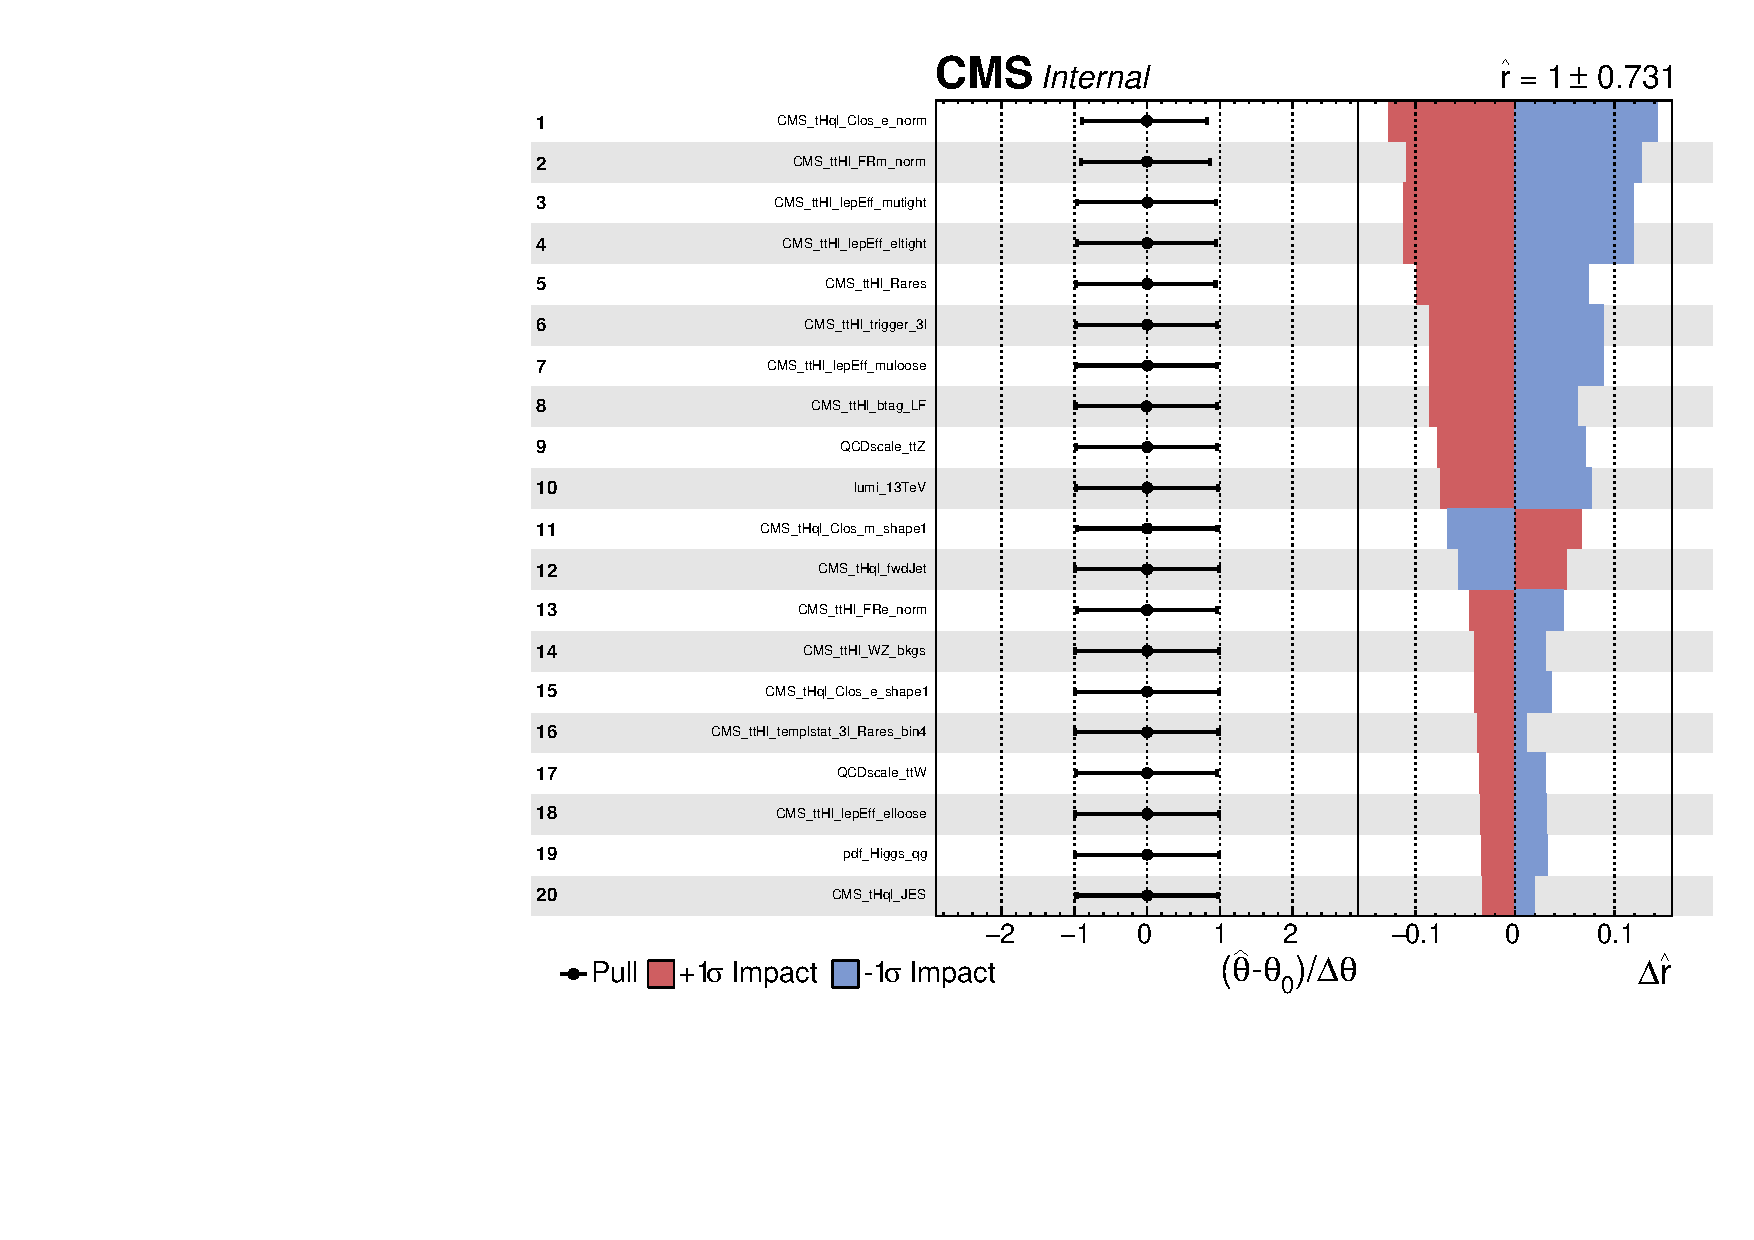
\includegraphics[width=1.0\textwidth]{figures/limits/impacts/impacts_40.pdf}\\
\caption{Post-fit pulls and impacts of the 20 nuisance parameters with $\pt$ cut $40$ GeV for the forward jet.}
\label{fig:impact40}
\end{figure}
